% import packages
\documentclass[12pt,a4paper]{article}
%\usepackage{times}
%\usepackage{wrapfig}
%\usepackage{latexsym}
%\usepackage{subcaption}
%\usepackage{csquotes}
%\usepackage{placeins}
%\usepackage{cleveref}
%\usepackage{setspace}
%\onehalfspacing
%\usepackage{array}
\usepackage{graphicx}
\usepackage{calc}
\usepackage{soul}
\usepackage[dvipsnames]{xcolor}
\usepackage[titles]{tocloft}
\usepackage{multirow}
\usepackage{booktabs}
\usepackage{threeparttable}
\usepackage{enumitem}
\usepackage{algorithm}
\usepackage{algpseudocode}
\usepackage{ragged2e}
\usepackage[hidelinks]{hyperref}
\usepackage[font=footnotesize]{caption}
\usepackage{csquotes}
\usepackage{float}
\usepackage[round,sort]{natbib}
\usepackage{tikz}
\usetikzlibrary{arrows,positioning,decorations.pathreplacing,shapes,calc,fit}
\usepackage{lipsum}
\usepackage{amsmath}
\usepackage{amssymb}
\usepackage{geometry}
\usepackage{url}
\usepackage{array,tabularx}
\usepackage{calc}

% define global variables
\newlength{\bibitemsep}\setlength{\bibitemsep}{.2\baselineskip plus .05\baselineskip minus .05\baselineskip}
\newlength{\bibparskip}\setlength{\bibparskip}{3pt}
\let\oldthebibliography\thebibliography
\renewcommand\thebibliography[1]{%
  \oldthebibliography{#1}%
  \setlength{\parskip}{\bibitemsep}%
  \setlength{\itemsep}{\bibparskip}%
}
\newlength{\DepthReference}
\settodepth{\DepthReference}{g}%relative to a depth of a letter.
\newlength{\HeightReference}
\settoheight{\HeightReference}{T}
\newlength{\Width}%
\newcommand{\MyColorBox}[2][red]%
{%
    \settowidth{\Width}{#2}%
    %\setlength{\fboxsep}{0pt}%
    \colorbox{#1}%
    {%      
        \raisebox{-\DepthReference}%
        {%
                \parbox[b][\HeightReference+\DepthReference][c]{\Width}{\centering#2}%
        }%
    }%
}
\setlength{\fboxsep}{1pt}
\setlength{\cftbeforesecskip}{1ex}
\colorlet{LightForestGreen}{ForestGreen!50!}
\colorlet{LightCyan}{Cyan!30!}
\renewcommand{\algorithmicrequire}{\textbf{Input:}}
\renewcommand{\algorithmicensure}{\textbf{Output:}}
\captionsetup[algorithm]{labelsep=colon}
\algnewcommand\algorithmicforeach{\textbf{for each}}
\algdef{S}[FOR]{ForEach}[1]{\algorithmicforeach\ #1\ \algorithmicdo}
\geometry{top=2.5cm,
		bottom=2.5cm}
\graphicspath{{img/}}
\newcommand\BibTeX{B\textsc{ib}\TeX}
%\renewcommand{\contentsname}{Table of Contents}
%\renewcommand{\refname}{Bibliography}
\newcolumntype{L}[1]{>{\RaggedRight\hspace{0pt}}p{#1}}
\newcolumntype{R}[1]{>{\RaggedLeft\hspace{0pt}}p{#1}}
\captionsetup[figure]{font=footnotesize,labelfont=footnotesize,labelfont={bf},labelformat={default},labelsep=period,name={Fig.}, justification=centering,singlelinecheck=false, width = \linewidth}
\captionsetup[table]{font=footnotesize,labelfont=footnotesize,labelfont={bf},labelformat={default},labelsep=period,name={Table},justification=centering, singlelinecheck=false, width = \linewidth}

% define admin variables
\title{Sentiment Analysis and Argumentation Mining in United
Nations Security Council Speeches}
\author{Juliane Hanel, Atreya Shankar\\
\texttt{\{hanel,shankar\}@uni-potsdam.de} \\
PM: Mining Sentiments and Arguments, WiSe 2019/20 \\
Prof. Dr. Manfred Stede \\
Applied Computational Linguistics\\
University of Potsdam}
\date{\today}

\begin{document}
\newgeometry{}
\maketitle
\thispagestyle{empty}
\begin{abstract}
The United Nations Security Council (UNSC) corpus from \citet{schnfeld2019security} is a novel political speech corpus containing $\sim$65,000 textual speech records from $\sim$5,000 security council meetings over the years of 1995-2017. Due to its large size and wide temporal distribution, it could be a very useful corpus for various Natural Language Processing (NLP) tasks in the political domain. One limitation of the current version of this corpus is its lack of extensive handwritten annotations; which diminish its utility for downstream supervised NLP tasks. In order to address this limitation, our project aims to evaluate and provide machine-driven sentiment and argumentation annotations for this corpus. We utilize state-of-the-art sentiment analysis and argumentation mining tools for this purpose, which include \texttt{VADER}, \texttt{AFINN}, and \texttt{TextBlob} for sentiment analysis and a political-domain fine-tuned version of the \texttt{ALBERT} language model for argumentation mining. Our automatic annotations, while not being as reliable as human annotations, nevertheless provide an initial foothold for future human annotations to follow-through.
\end{abstract}
\newpage
\restoregeometry
\thispagestyle{empty}
\tableofcontents
\newpage
\setcounter{page}{1}
\thispagestyle{plain}
\section{Introduction}

The United Nations Security Council (UNSC) corpus, detailed in \citet{schnfeld2019security}, is a novel political speech corpus containing 65,393 textual speech records from 4,460 security council meetings over the years of 1995-2017. Due to its large size and wide temporal distribution, it could be a very useful corpus for various Natural Language Processing (NLP) tasks in the political domain.

One limitation of the current version of this corpus is its lack of extensive handwritten annotations \citep{schnfeld2019security}; which diminishes its utility for downstream supervised NLP tasks. In order to address this limitation, our project aims to evaluate and provide machine-driven sentiment and argumentation annotations for this corpus. We utilize state-of-the-art tools for this purpose, which include \texttt{VADER}, \texttt{AFINN}, and \texttt{TextBlob} for sentiment analysis and a political-domain fine-tuned version of the \texttt{ALBERT} language model for argumentation mining. Our automatic annotations, while not being as reliable as human annotations, nevertheless provide an initial foothold for future human annotations to follow-through.

In section \ref{background}, we describe and define various background concepts that are used for the methodologies in this paper. In section \ref{methods}, we describe the various methodologies implemented in this study. In sections \ref{results} and \ref{discuss}, we describe our results and discuss their implications. Lastly, we conclude this study in section \ref{conclu} and provide some recommendations for future work in section \ref{reco}.
\section{Background Concepts}
\label{background}

\subsection{United Nations Security Council (UNSC) Corpus}
As the UNSC corpus was already briefly described in the introduction, we will proceed to describe some key statistics regarding this corpus. As mentioned, this corpus contains textual data from 65,393 speeches which were collected from 1995-2017. In Figure \ref{UNSC_stats_1}, we can observe how the number of speeches and meetings vary temporally. We can, for example, notice how there was a peak in the number of speeches per meeting in 2003; which corresponds to the onset of the Iraq war.

\begin{figure}[H]
    \centering
    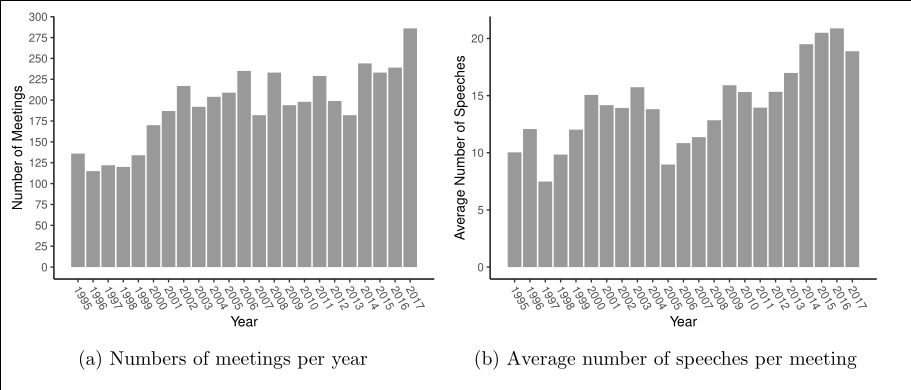
\includegraphics[trim={0.2cm 0.1cm 0 0.1cm},clip,width=\textwidth]{unsc_speeches_stats_1.png}
    \caption{Temporal distribution of the number of speeches and meetings in the UNSC corpus \citep{schnfeld2019security}}
    \label{UNSC_stats_1}
\end{figure}

\begin{figure}[t]
    \centering
    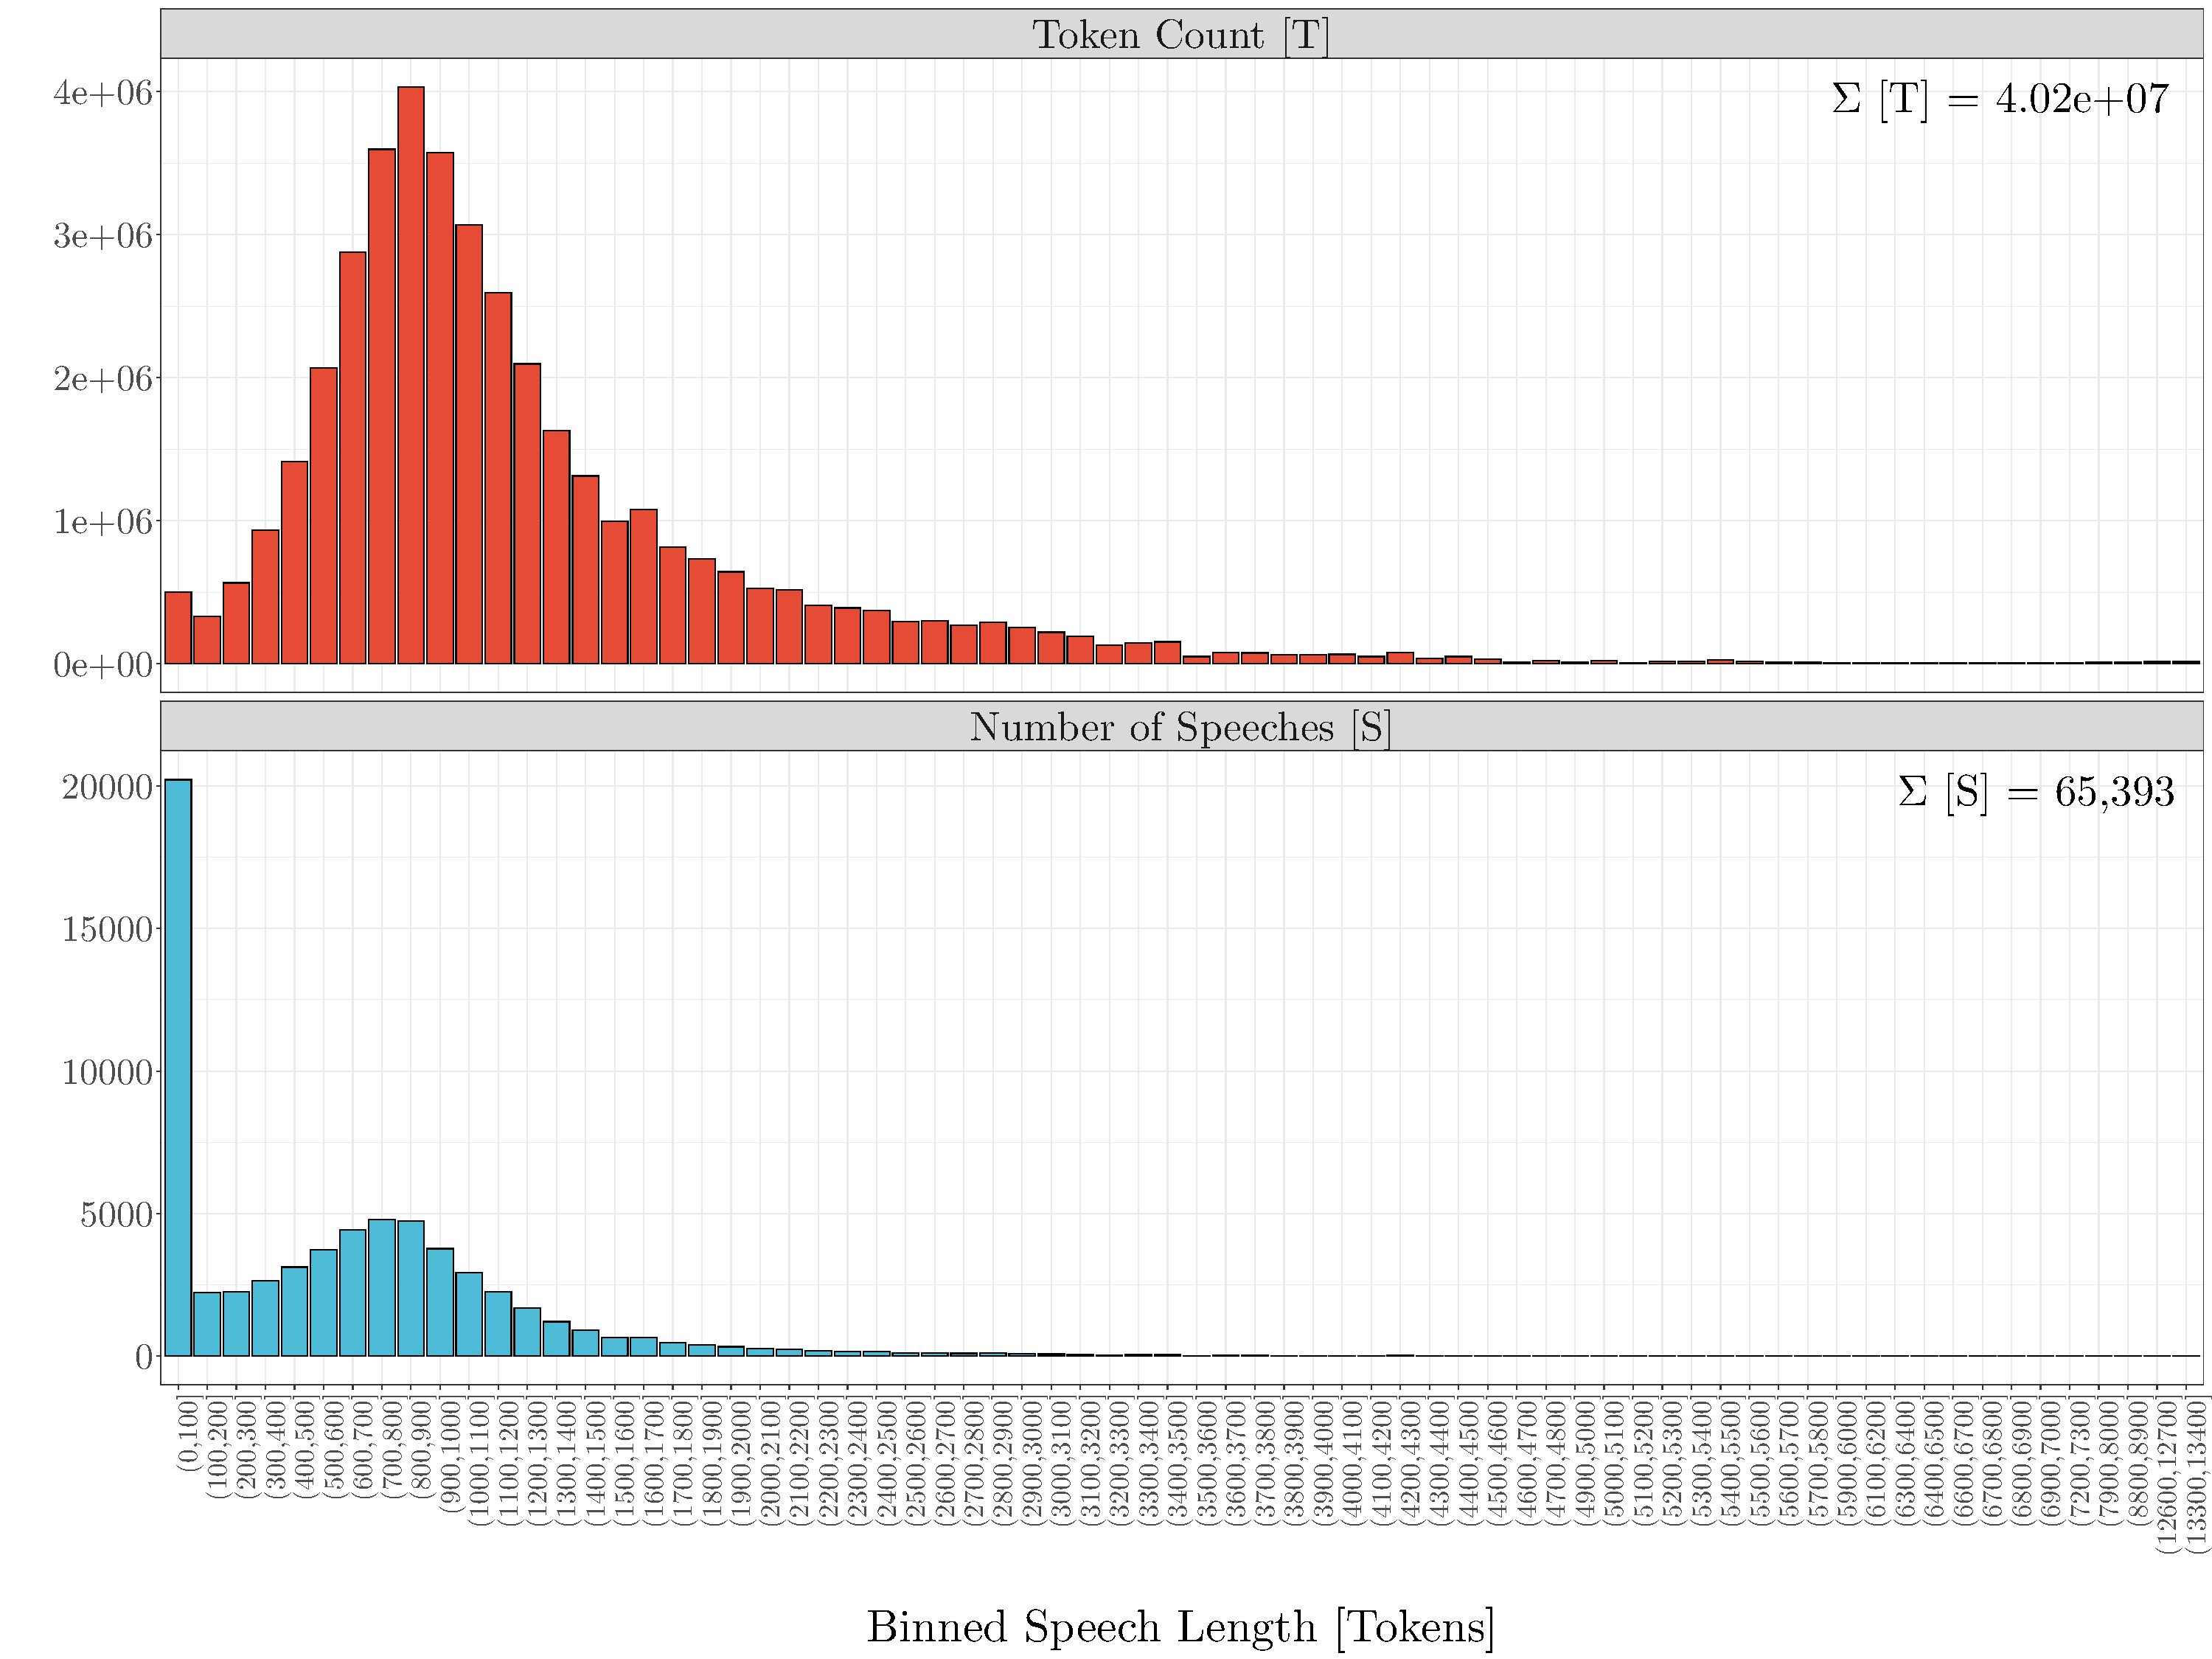
\includegraphics[trim={1.1cm 0.1cm 0 0.1cm},clip,width=\textwidth]{token_dist_UNSC_length.pdf}
    \caption{Token count (top; red) and number of speeches (bottom; blue) by binned speech length in the UNSC corpus}
    \label{UNSC_stats_2}
\end{figure}

To get a better idea of the token statistics of the UNSC speeches, we conducted a simple tokenization and binning procedure on the corpus. Here, we removed certain redundant parts of each speech, such as the initial tokens describing which speaker is speaking. Then we tokenized the left-over speeches using the \texttt{nltk} python module. After this, we binned all of the speeches by their token lengths into intervals of 100 tokens, and plotted the number of tokens and speeches in each binned category as shown in Figure \ref{UNSC_stats_2}.

Here, we can observe that the number of speeches peaks at the binned speech length category of \texttt{(0,100]}, while the number of tokens peaks at the binned speech length category of \texttt{(800,900]} tokens. This tells us that most of the UNSC speeches are generally short and have a length less than or equal to 100 tokens, but the majority of tokens are found in longer length speeches between 800 and 900 tokens. This information will come into further use in later parts of this paper.

\subsection{Sentiment Analysis}

According to \citet{liu2012sentiment}:

\begin{displayquote}
``Sentiment analysis and opinion mining is the field of study that analyzes people's opinions, sentiments, evaluations, attitudes, and emotions from written language. It is one of the most active research areas in natural language processing and is also widely studied in data mining, Web mining, and text mining."
\end{displayquote}

Sentiment analysis can be used to detect various sentiment polarities, for example detecting if a given utterance is positive/negative or subjective/objective \citep{liu2012sentiment}. In such cases, the sentiment value of an utterance typically takes on a real value from --1 to +1, where each extremum indicates one of the polarities of interest. Furthermore, sentiment analysis can be conducted on various granularities or scales \citep{liu2012sentiment}. These can range from a sentence level to a document level and can include various user-defined aspects. For example, given a certain online product review, sentiment analysis could decipher the sentiment polarity towards aspects such as service, product quality and delivery time.

In this paper, we will generally be dealing with sentiment analyses of entire UNSC speeches. This would therefore correspond to sentiment analysis on a document level. In the next subsections, we will proceed to describe some commonly used automatic sentiment analysis tools.

\subsubsection{VADER}

The Valence Aware Dictionary for Sentiment Reasoning (VADER) is a simple rule-based model for general sentiment analysis of social media text \citep{vader}. VADER utilizes a generalized valence-based and human-curated sentiment lexicon to score utterances for their sentiment polarity. Since it was created from handcrafted rules, the VADER sentiment analysis system does not have training data. However, it has been evaluated on various sentiment datasets and shows high classification accuracy; as well as a strong correlation to human-annotator performance \citep{vader}.

VADER has different scoring regimes for sentiment polarities of utterances. Table \ref{table_vader} gives a summary of the various VADER sentiment scores.

\begin{table}[H]
	\centering
	\small
	\setlength{\tabcolsep}{0.5em}
	\def\arraystretch{1.1}
	\begin{threeparttable}
		\begin{tabular}{L{0.2\linewidth} p{0.75\linewidth}}
			\toprule[0.25mm]
			Scores & Description \\
			\midrule[0.35mm]
			\multirow{3}{*}{\shortstack[l]{Positive \\[3pt] Negative \\[3pt] Neutral}}  & All three of these scores refer to the proportion of the input text that is positive, negative or neutral. Ultimately, the sum of the positive, negative and neutral scores must add up to 1. \\[35pt]
			Compound  & The compound score is computed by adding the polarity scores of each word in the sentiment lexicon, adjusted according to the rules, and then normalized between --1 (most extreme negative) and +1 (most extreme positive). One can refer to the compound score as a normalized and weighted composite sentiment score.\\[20pt]
			\bottomrule[0.25mm]
		\end{tabular}
		\caption{Tabular summary of VADER sentiment scores}
		\label{table_vader}
	\end{threeparttable}
\end{table}

One limitation of VADER is that it was constructed to perform on ``microblog-like" contexts found typically on social media platforms such as \textit{Twitter}. However, \citet{vader} do state that VADER is a robust tool and can perform well on diverse domains. For this reason, we consider VADER as a feasible sentiment analysis tool for the UNSC corpus.

\subsubsection{AFINN}
AFINN is a widely used multilingual lexicon containing words and their valence, manually rated between -5 and +5. For sentence-wise rating, the valence of the words is simply aggregated. The latest version of the English AFINN lexicon\footnote{\href{https://github.com/fnielsen/afinn/blob/master/afinn/data/AFINN-en-165.txt}{https://github.com/fnielsen/afinn/blob/master/afinn/data/AFINN-en-165.txt}} contains more than 3,300 words.
The author, Finn Nielsen, has created a Python wrapper called \texttt{afinn} that grants programmers easy access to the lexicon \citep{afinn}.
Despite its simplicity, AFINN performs very well on various tasks in benchmark testing \citep{sentibench}. 
Due to its extensive and relatively unbiased contents, we consider AFINN to be a valuable addition to VADER. The compound scores VADER provides give an idea of the document-level sentiment in the UNSC speeches. For sentence-wise rating, we will rely on AFINN.

\subsubsection{TextBlob}

\texttt{TextBlob} is a python library used for processing textual data. This library also incorporates a successful lexical sentiment analysis tool, which is inherited from the \texttt{pattern} python library. TextBlob's default sentiment analyzer, known as \texttt{PatternAnalyzer}, works in a similar way compared to VADER and assigns sentiment scores to relevant words using a manually annotated sentiment lexicon \citep{smedt2012pattern}. It then averages the lexical sentiment scores to create an overall sentiment score. Table \ref{table_textblob} gives a summary of the two types of scores that this tool can output.

\begin{table}[H]
	\centering
	\small
	\setlength{\tabcolsep}{0.5em}
	\def\arraystretch{1.1}
	\begin{threeparttable}
		\begin{tabular}{L{0.2\linewidth} p{0.75\linewidth}}
			\toprule[0.25mm]
			Scores & Description \\
			\midrule[0.35mm]
			Polarity & This score takes on real-values from --1 to +1, where --1 indicates negative while +1 indicates positive sentiment polarity. \\[20pt]
			Subjectivity  & This score takes on real-values from 0 to +1, where 0 indicates an objective utterance while +1 indicates a subjective utterance.\\[10pt]
			\bottomrule[0.25mm]
		\end{tabular}
		\caption{Tabular summary of TextBlob \texttt{PatternAnalyzer} sentiment scores}
		\label{table_textblob}
	\end{threeparttable}
\end{table}

\subsection{Argumentation Mining}

According to \citet{van2004systematic}:

\begin{displayquote}
``Argumentation is a verbal, social, and rational activity aimed at convincing a reasonable critic of the acceptability of a standpoint by putting forward a constellation of propositions justifying or refuting the proposition expressed in the standpoint."
\end{displayquote}

Argumentation mining can be defined as the process of decomposing text into Argumentative Discourse Units (ADUs) and connecting these units into a comprehensive argumentation tree, where an ADU is defined as the \textit{``span of text that plays a single role for the argument being analyzed, and is demarcated by neighboring text spans that play a different role, or none at all"} \citep{stede2018argumentation}. We will expound further on corpus-specific ADUs and argumentation trees in section \ref{corpora}. \citet{stede2018argumentation} further provide an exhaustive overview for the process of argumentation mining (not necessarily in numerical order):

\begin{enumerate}
    \item Identify argumentative text (or a portion of a text)
    \item Segment the text into ADUs
    \item Identify the central claim
    \item Identify the role/function of ADUs
    \item Identify relations between ADUs
    \item Build the overall structural representation or argumentation tree
    \item Identify the type and the quality of the argumentation
\end{enumerate}

It is worth noting that there exist significant differences in the granularities of ADUs and their corresponding argumentation trees depending on the corpus of reference. Some corpora, such as the argumentative microtext corpus detailed in \citet{peldszus2015annotated}, go into deep detail regarding the relationships between ADUs; specifying central claims, support/attack segments and even describing subtypes of these ADUs, as seen in Figure \ref{args_structure}. Other corpora, such as the US Election Debate corpus detailed in \citet{haddadan-etal-2019-yes}, go into less detail and simply identify ADUs as claims or premises; and only specify basic hierarchies to build an argumentation tree.

Overall, argumentation mining provides the ability to automatically extract important information on the argumentative components of text. This process is extremely valuable for downstream NLP tasks which require distilled information; such as text summarization and question answering.

\begin{figure}[t]
    \centering
    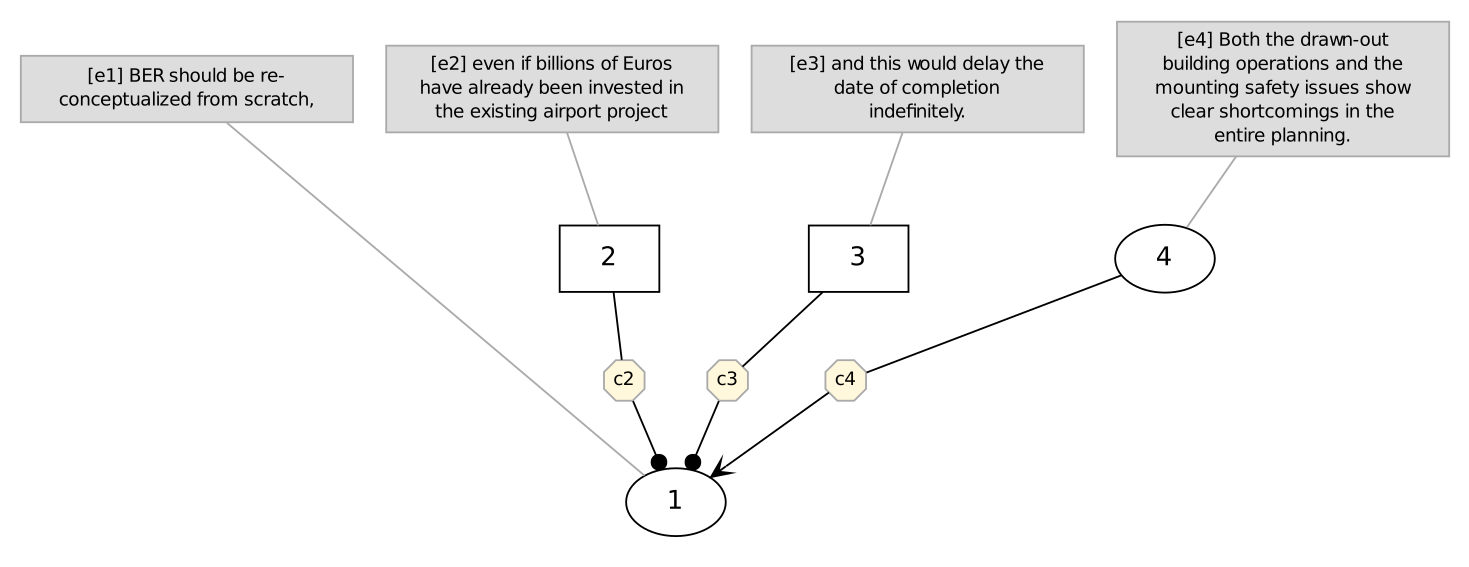
\includegraphics[trim={0cm 0cm 0 0cm},clip,width=\textwidth]{args_structure.png}
    \caption{Sample argumentation tree from argumentative microtext corpus detailed in \citet{peldszus2015annotated}; bottom-most node represents the central claim; arrow-head represents supporting ADU; circle represents attacking ADU}
    \label{args_structure}
\end{figure}

\subsubsection{Copora}
\label{corpora}

As mentioned previously, the granularities of ADUs and the complexity of argumentation trees are usually dependent on the corpus of reference. Table \ref{table_arg_corpora} shows a summary of three high-quality annotated argumentation corpora that are available to the public. Since the ultimate aim of this study is to apply an argumentation classifier on the UNSC corpus, it would make sense to select a well-suited argumentation corpus in order to train a relevant argumentation classifier.

Referring back to Figure \ref{UNSC_stats_2}, we can observe that the UNSC corpus has a wide distribution of speech token lengths. In order to be similar to the UNSC corpus, a well-suited annotated argumentation corpus should have the following properties:

\begin{enumerate}
    \item Relatively long sequence lengths similar to the UNSC corpus; which has a mean sequence length of $\sim$600 tokens.
    \item Sufficiently large number of training data instances with negative (non-argumentative) examples to robustly train an argumentation classifier.
    \item If possible, the corpus should exist in the political domain in order to maximize domain similarity.
    \item If possible, utilize newly published corpus to contribute to research findings.
\end{enumerate}

Given these requirements, points 2, 3, and 4 are satisfied best by the US Election Debate (USED) corpus. Point 1 is best satisfied by the persuasive essay corpus. However, as a mitigating factor towards point 1, the USED corpus has a very large standard deviation to mean ratio in its sequence length; which implies that there are many data instances which are also longer in length.

\begin{table}[t]
	\centering
	\small
	\setlength{\tabcolsep}{0.5em}
	\def\arraystretch{1.1}
	\begin{threeparttable}
		\begin{tabular}{L{0.22\linewidth} L{0.11\linewidth} L{0.17\linewidth} p{0.39\linewidth}}
			\toprule[0.25mm]
			Annotated \qquad Argumentation Corpus & Data \qquad Instances & Seq. Length Statistics \qquad [Tokens]$^{\dagger}$ & \multicolumn{1}
			{L{0.39\linewidth}}{ADU Granularity and \qquad \qquad Argumentation Tree \qquad \qquad Complexity} \\[25pt]
			\midrule[0.35mm]
			Argumentative microtext corpus \citep{peldszus2015annotated} & 
			112 \qquad texts &  $\begin{aligned}[t] % placement: default is "center", options are "top" and "bottom"
\overline{X} &= 78.2\\
\hat{\sigma} &= 21.5
\end{aligned}$& Fine-grained ADUs with support/attack nature and subtypes, complex argumentation trees \\\\[-5pt]
			Persuasive essay corpus \citep{stab2017parsing} & 402 \qquad \qquad essays & $\begin{aligned}[t] % placement: default is "center", options are "top" and "bottom"
\overline{X} &= 366.0\\
\hat{\sigma} &= 62.9
\end{aligned}$ & Fine-grained ADUs with support/attack nature, complex argumentation trees \\\\[-5pt]
			US election debate corpus \citep{haddadan-etal-2019-yes} & 6,559 speech turns & $\begin{aligned}[t] % placement: default is "center", options are "top" and "bottom"
\overline{X} &= 110.4\\
\hat{\sigma} &= 151.6
\end{aligned}$ & Coarse ADUs as either claims or premises, simple argumentation trees \\[25pt]
			\bottomrule[0.25mm]
		\end{tabular}
    \begin{tablenotes}[flushleft]
      \scriptsize
      \item $^{\dagger}\overline{X}$ and $\hat{\sigma}$ represent the sample mean and standard deviations of sequence token lengths
    \end{tablenotes}
		\caption{Tabular summary of three prospective annotated argumentation corpora}
		\label{table_arg_corpora}
	\end{threeparttable}
\end{table}

\subsubsection{Models}
\label{models}

In order to gain information about state-of-the-art argumentation classification models, we conducted a survey based on recent publications and summarized key information on three models in Table \ref{table_arg_models}. Since these models were published in or before 2019, we can observe that they were trained/evaluated on the persuasive essay and argumentative microtext corpora, and not the USED corpus due to it only being released in mid-2019.

Furthermore, we can observe that both \citet{potash2016heres} and \cite{kuribayashi2019empirical} train their argumentation classifiers on the assumption that ADU spans in text are pre-defined. This, while being a reasonable assumption for partially annotated text, is not a sound assumption for non-annotated text where there exist no pre-defined ADU spans, as is the case for the UNSC corpus.

This limitation was in fact noted by \citet{eger2017neural}, which perhaps inspired them to create a more ground-up methodology of conducting sequence tagging in order to classify ADU spans, types and linkages altogether as a joint task. This technique of sequence tagging to form a ground-up framework is notable and will be revisited in section \ref{fine_tune} of this study.

Another limitation of all three models is their language encoding techniques. Recent developments in NLP have shown that transformer-based language models, such as BERT, far outperform other language encodings such as Bag-of-Words, GloVe and ELMo \citep{devlin2018bert}. Exploring new BERT-style language encodings could be an interesting avenue to further our research.

\begin{table}[t]
	\centering
	\small
	\setlength{\tabcolsep}{0.5em}
	\def\arraystretch{1.1}
	\begin{threeparttable}
		\begin{tabular}{L{0.19\linewidth} L{0.10\linewidth} L{0.20\linewidth} L{0.17\linewidth} L{0.21\linewidth}}
			\toprule[0.25mm]
			Model & Corpus$^{\dagger}$ & Task & Language \qquad Encoding & Best Performance \qquad [Macro-F$_1$]$^{\ddagger}$ \\
			\midrule[0.35mm]
			Joint Pointer \qquad Network \citep{potash2016heres} & PEC \qquad MTC & Classify ADU types and linkages given pre-defined spans & Bag-of-Words \qquad GloVe & PEC: 0.801 \qquad \qquad MTC: 0.777 \\\\[-5pt]
			BLCC tagger and LSTM-ER \citep{eger2017neural} & PEC & Sequence tagging for ADU spans, types and linkages & GloVe & Exact: 0.449  \qquad Half-span: 0.505 \\\\[-5pt]
			Span-based \qquad BiLSTM \citep{kuribayashi2019empirical} & PEC \qquad MTC & Classify ADU types and linkages given pre-defined spans & GloVe \qquad ELMo & PEC: 0.818 \qquad \qquad MTC: 0.782 \\[20pt]
			\bottomrule[0.25mm]
		\end{tabular}
    \begin{tablenotes}[flushleft]
      \scriptsize
      \item $^{\dagger}$PEC: Persuasive Essay Corpus, MTC: Argumentative Microtext Corpus
      \item $^{\ddagger}$Where necessary, F$_1$ scores were averaged amongst joint tasks for brevity
    \end{tablenotes}
		\caption{Tabular summary of three state-of-the-art argumentation classification models}
		\label{table_arg_models}
	\end{threeparttable}
\end{table}

\subsection{Transformer-Based Language Models}

Since the introduction of the transformer architecture in the iconic ``Attention is all you need" paper by \citet{vaswani2017attention}, we have seen the transformer architecture being used extensively in various NLP tasks, particularly in unsupervised language encoding. Transformers show significant advantages over traditional recurrent encoder-decoder frameworks due to their self-attention mechanism; which has shown to both increase performance, and efficiency through improved parallelization \citep{vaswani2017attention}.

Since previous argumentation models shown in Table \ref{table_arg_models} did not leverage on state-of-the-art transformer architectures, it could be a good addition for us to conduct our research using such transformer architectures.

\subsubsection{BERT}
\label{bert}

BERT, which abbreviates Bidirectional Encoder Representations from Transformers, is a novel context-aware language model trained using transformers \citep{devlin2018bert}. After pre-training on unsupervised language modeling tasks, BERT can be fine-tuned for downstream NLP tasks such as question-answering and natural entity recognition \citep{devlin2018bert}. A schematic for this process can be seen in Figure \ref{bert_schematic}. Fine-tuning BERT on various NLP tasks has shown significant performance improvements over preceding baselines; which is a large factor for recent academic interest and publications regarding the model.

\begin{description}[style=nextline]
\item [Architecture] In \citet{devlin2018bert}, two variants of BERT known as BERT$_{\text{BASE}}$ ($L=12$, $H=768$, $A=12$, $P=110$ million) and BERT$_{\text{LARGE}}$ ($L=24$, $H=1024$, $A=16$, $P=340$ million) were tested; where $L$ refers to the number of transformer blocks, $H$ refers to the hidden size, $A$ refers to the number of self-attention heads and $P$ refers to the total number of parameters. The models were trained on 4 and 16 Cloud TPUs respectively, training for a total of 4 days.

\begin{figure}[t]
    \centering
    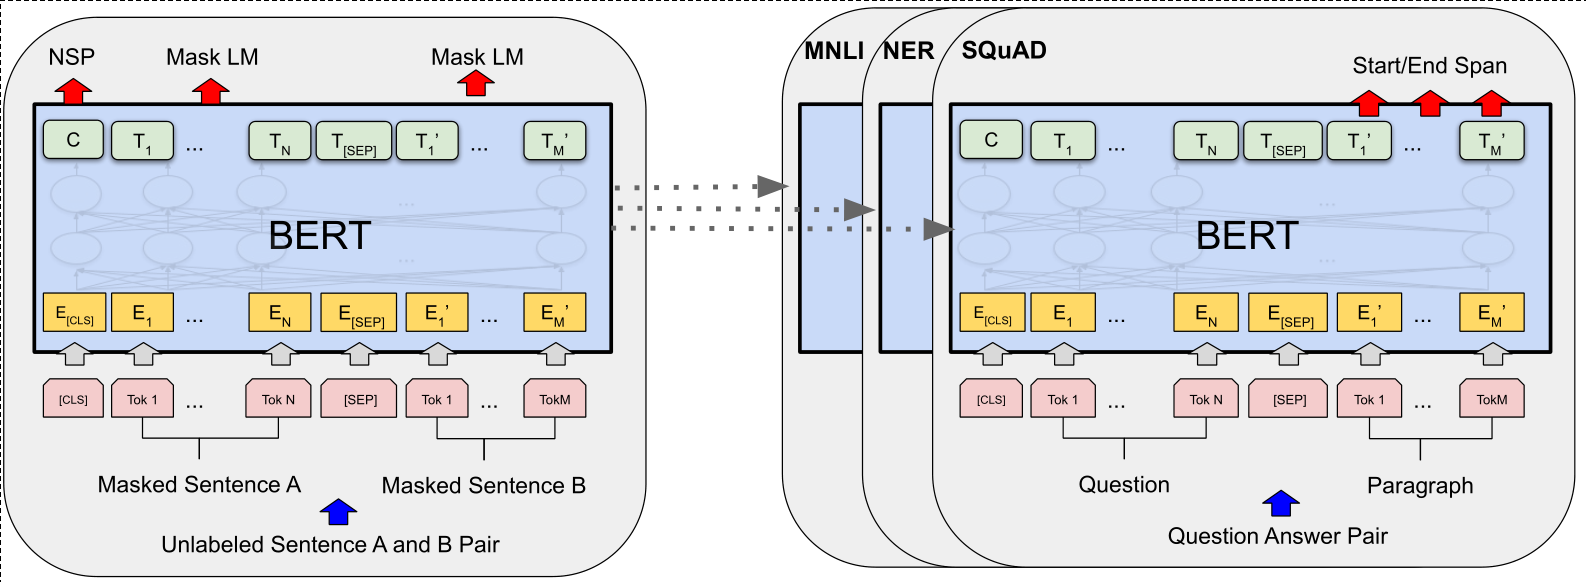
\includegraphics[trim={0.1cm 0cm 0cm 0.1cm},clip,width=\textwidth]{bert_schematic.png}
    \caption{Schematic of BERT pre-training (left) and fine-tuning (right) for downstream NLP tasks \citep{devlin2018bert}}
    \label{bert_schematic}
\end{figure}

\item [Pre-training Tasks] BERT was trained with two pre-training objectives; namely Masked Language Model (MLM) and Next Sentence Prediction (NSP). Under the MLM task, some percentage of input tokens are masked at random and the model is trained to predict the identities of the masked tokens. This task incorporates a global context of the input text, since all of the context would be necessary to predict the masked token(s). Under NSP, some consecutive sentences are shuffled at random and BERT learns to predict whether sentence B indeed follows sentence A. Through this process, BERT incorporates sequential context for natural language understanding and this pre-training task has been shown to help with downstream NLP tasks such as question-answering.

\item [Special Tokens] BERT incorporates certain special tokens in order to perform the aforementioned pre-training tasks; namely \texttt{[CLS]}, \texttt{[SEP]}, \texttt{<pad>} and \texttt{<unk>}. The \texttt{[CLS]} token is found at the start of every sequence and its position in the model output represents the aggregate representation of the entire sequence; which is why this token's position is used for sequence classification tasks. The \texttt{[SEP]} token is a separator token which is used to separate sentence pairs for the NSP pre-training task. \citet{devlin2018bert} also suggests that the \texttt{[SEP]} token should be used at the end of sequences; although there are some discrepancies regarding this in their paper. For simplicity, we assume that the \texttt{[SEP]} token should additionally be placed at the end of input sequences. The \texttt{<pad>} and \texttt{<unk>} tokens represent padding and unknown tokens respectively. BERT additionally enforces a maximum input sequence length of 512 tokens.

\item [WordPiece Tokenization] BERT uses the WordPiece Model (WPM) for tokenization of its input text. The WPM is a novel and powerful tokenization model that tokenizes words into sub-word units \citep{wu2016google}. This is a powerful approach as it mitigates the large vocabularies and out-of-vocabulary (OOV) issues of purely word-based tokenizers, as well as the small vocabularies and semantic information loss of purely character-based tokenizers. Following is an example of the WPM model's output, which has been adapted from \citet{wu2016google}:

\begin{description}
    \item [Input Sequence:] Jet makers feud over seat widths
    \item [WordPiece Output:] $\_$J et $\_$makers $\_$fe ud $\_$over $\_$seat $\_$width s
\end{description}

``$\_$" is a special character used to mark the beginning of a word. A token which does not start with ``$\_$" is a segmented sub-word of a main word; for example ``et" being a sub-word of ``Jet" in the example above. It is worth noting here that a combination of using the WPM and special tokens in BERT result in input sequences becoming much longer than they originally were. As a result, some input sequences in corpora might exceed BERT's 512 token hard upper-limit and might need to be discarded from analysis.

\item [Fine-tuning] For pre-training BERT, large unsupervised corpora such as BookCorpus (800 million words) and English Wikipedia (2,500 million words) are used \citep{devlin2018bert}. Fine-tuning follows after pre-training and involves slightly adjusting all the parameters in BERT in order to perform on downstream NLP tasks and corresponding supervised corpora. Compared to pre-training, fine-tuning is relatively fast and computationally inexpensive \citep{devlin2018bert}. Fine-tuning BERT on downstream NLP tasks has shown significant improvements in state-of-the-art performances, which include a 7.7$\%$ point absolute improvement of the GLUE score for the General Language Understanding Evaluation (GLUE) task.
\end{description}

\subsubsection{ALBERT}
\label{albert}

\begin{figure}[t]
    \centering
    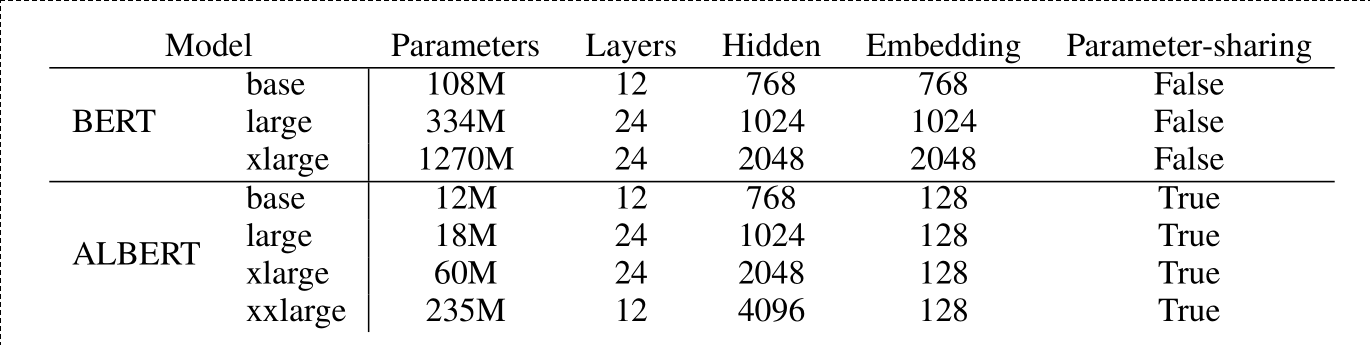
\includegraphics[trim={0.2cm 0cm 0cm 0.2cm},clip,width=\textwidth]{img/albert_comparison.png}
    \caption{Tabular excerpt from \citet{lan2019albert} on BERT vs. ALBERT architecture}
    \label{albert_comparison}
\end{figure}

A major criticism of the aforementioned BERT language model is its sheer size in terms of parameters; which can ultimately lead to GPU/TPU memory limitations, long training times and unexpected model degradation. To address these issues, \citet{lan2019albert} propose a ``lite" version of BERT (a.k.a. ALBERT) which utilizes factorized embedding parameterization and cross-layer parameter sharing to reduce memory consumption and increase training speed. Figure \ref{albert_comparison} shows how this optimization results in a drop in the number of parameters in the ALBERT model(s); for example the ALBERT$_{\text{BASE}}$ model can be reduced to 12 million parameters, making it a suitable candidate to train even on a single GPU.

To further improve performance, \citet{lan2019albert} replace the NSP task in BERT's unsupervised pre-training with a sentence-order prediction (SOP) task. This involves the same task as per NSP for positive examples. However, negative examples involve two consecutive sentences being swapped in terms of their order. According to \citet{lan2019albert}, the SOP task pushes ALBERT to learn more fine-grained distinctions on discourse-level coherence properties. This modification has shown to improve downstream NLP task performance for multi-sentence problems. Additionally, ALBERT uses the SentencePiece tokenization model (SPM) from \citet{kudo2018sentencepiece}, which incorporates the Unigram Language Model (ULM) from \citet{kudo2018subword}. The SPM is similar to BERT's WPM, but is purportedly faster and more versatile compared to the WPM.

Despite these key differences, ALBERT is still very similar to BERT in terms of its general architecture and building blocks, which can be seen as well in Figure \ref{albert_comparison}. Additionally, it is worth noting that the 512 token hard upper-limit for input sequences also applies for ALBERT. Ultimately, since ALBERT has shown to both perform and scale better than its BERT counterpart (with particular focus on discourse-level coherence for its SOP task), we consider ALBERT as a viable model for use in our argumentation mining task. This application will be further expounded on in section \ref{fine_tune} of our study.
\section{Methodologies}
\label{methods}

\subsection{Sentiment Analysis}
\subsubsection{Data Preprocessing}
For conducting the sentiment analysis, preprocessing of the data was necessary. Since the 65,393 speeches contained in the corpus were provided as separate text files, we decided to combine the speeches for each year, allowing for an analysis of the sentiment development over time. 
We resolved several issues that arose in the process, e.g. duplicate speech IDs or missing meta data. 

The yearly overview used for the analysis included the speech ID, date, speech text, cleaned text, topic, country, name of the speaker, participant type, subjectivity score, sentiment score, number of positive sentences, and number of negative sentences for each speech.

In order to perform inter- and intracountry comparisons, we calculated the yearly average for each feature (i.e. sentiment, subjectivity, positive and negative sentences) for each country. Using this average data, we also calculated the standard deviation of the scores for each country over time. 

We also created additional overviews for analyzing the the core nations of the UNSC, the sentiment of the core nations related to the Iraq War. Lastly, we created two more overviews for a detailed country-level sentiment analysis during two specific resolutions related to the invasion of Iraq. 

After creating these data overviews in Python, we stored each one locally as \texttt{csv} file since computation on each access of the data would have been too costly. For the purpose of easy access, we prepared several helper functions which load the data into the Python data structure \texttt{Pandas DataFrame}. We chose the DataFrame for data storage and manipulation since it efficiently handles large data and is much more flexible than standard data structures.

\subsubsection{Sentiment Polarity and Subjectivity}

As mentioned in section 2.2.1, we relied on commonly used automatic sentiment analysis tools for our analysis.  As for the processing of the speeches for this analysis, we chose to clean the speeches, which means that we removed stop words (common words with no inherent meaning) and transformed the text into lowercase. This was done for the sentiment analysis using VADER and the subjectivity analysis using TextBlob. For the calculation of the amount of positive and negative sentences per speech with AFINN, we also tokenized the words in the speeches. Tokenization yielded no improved results for sentiment and subjectivity analysis. For text manipulation, we used the Python \texttt{nltk} library.

As for the visualizations of the analysis results, we relied on Python's \texttt{matplotlib} plotting library, expanded with the \texttt{Seaborn} library. All analyses and data handling was performed with \texttt{Python 3.7.4}.  Our final product for sentiment analysis is a human-readable \texttt{json} file mapping UNSC speech IDs to sentiment and subjectivity scores, available in our public GitHub repository\footnote{https://github.com/atreyasha/sentiment-argument-mining}.

\subsection{Argumentation Mining}
\subsubsection{US Election Debate Corpus}
\label{used}

\begin{figure}[b!]
    \centering
    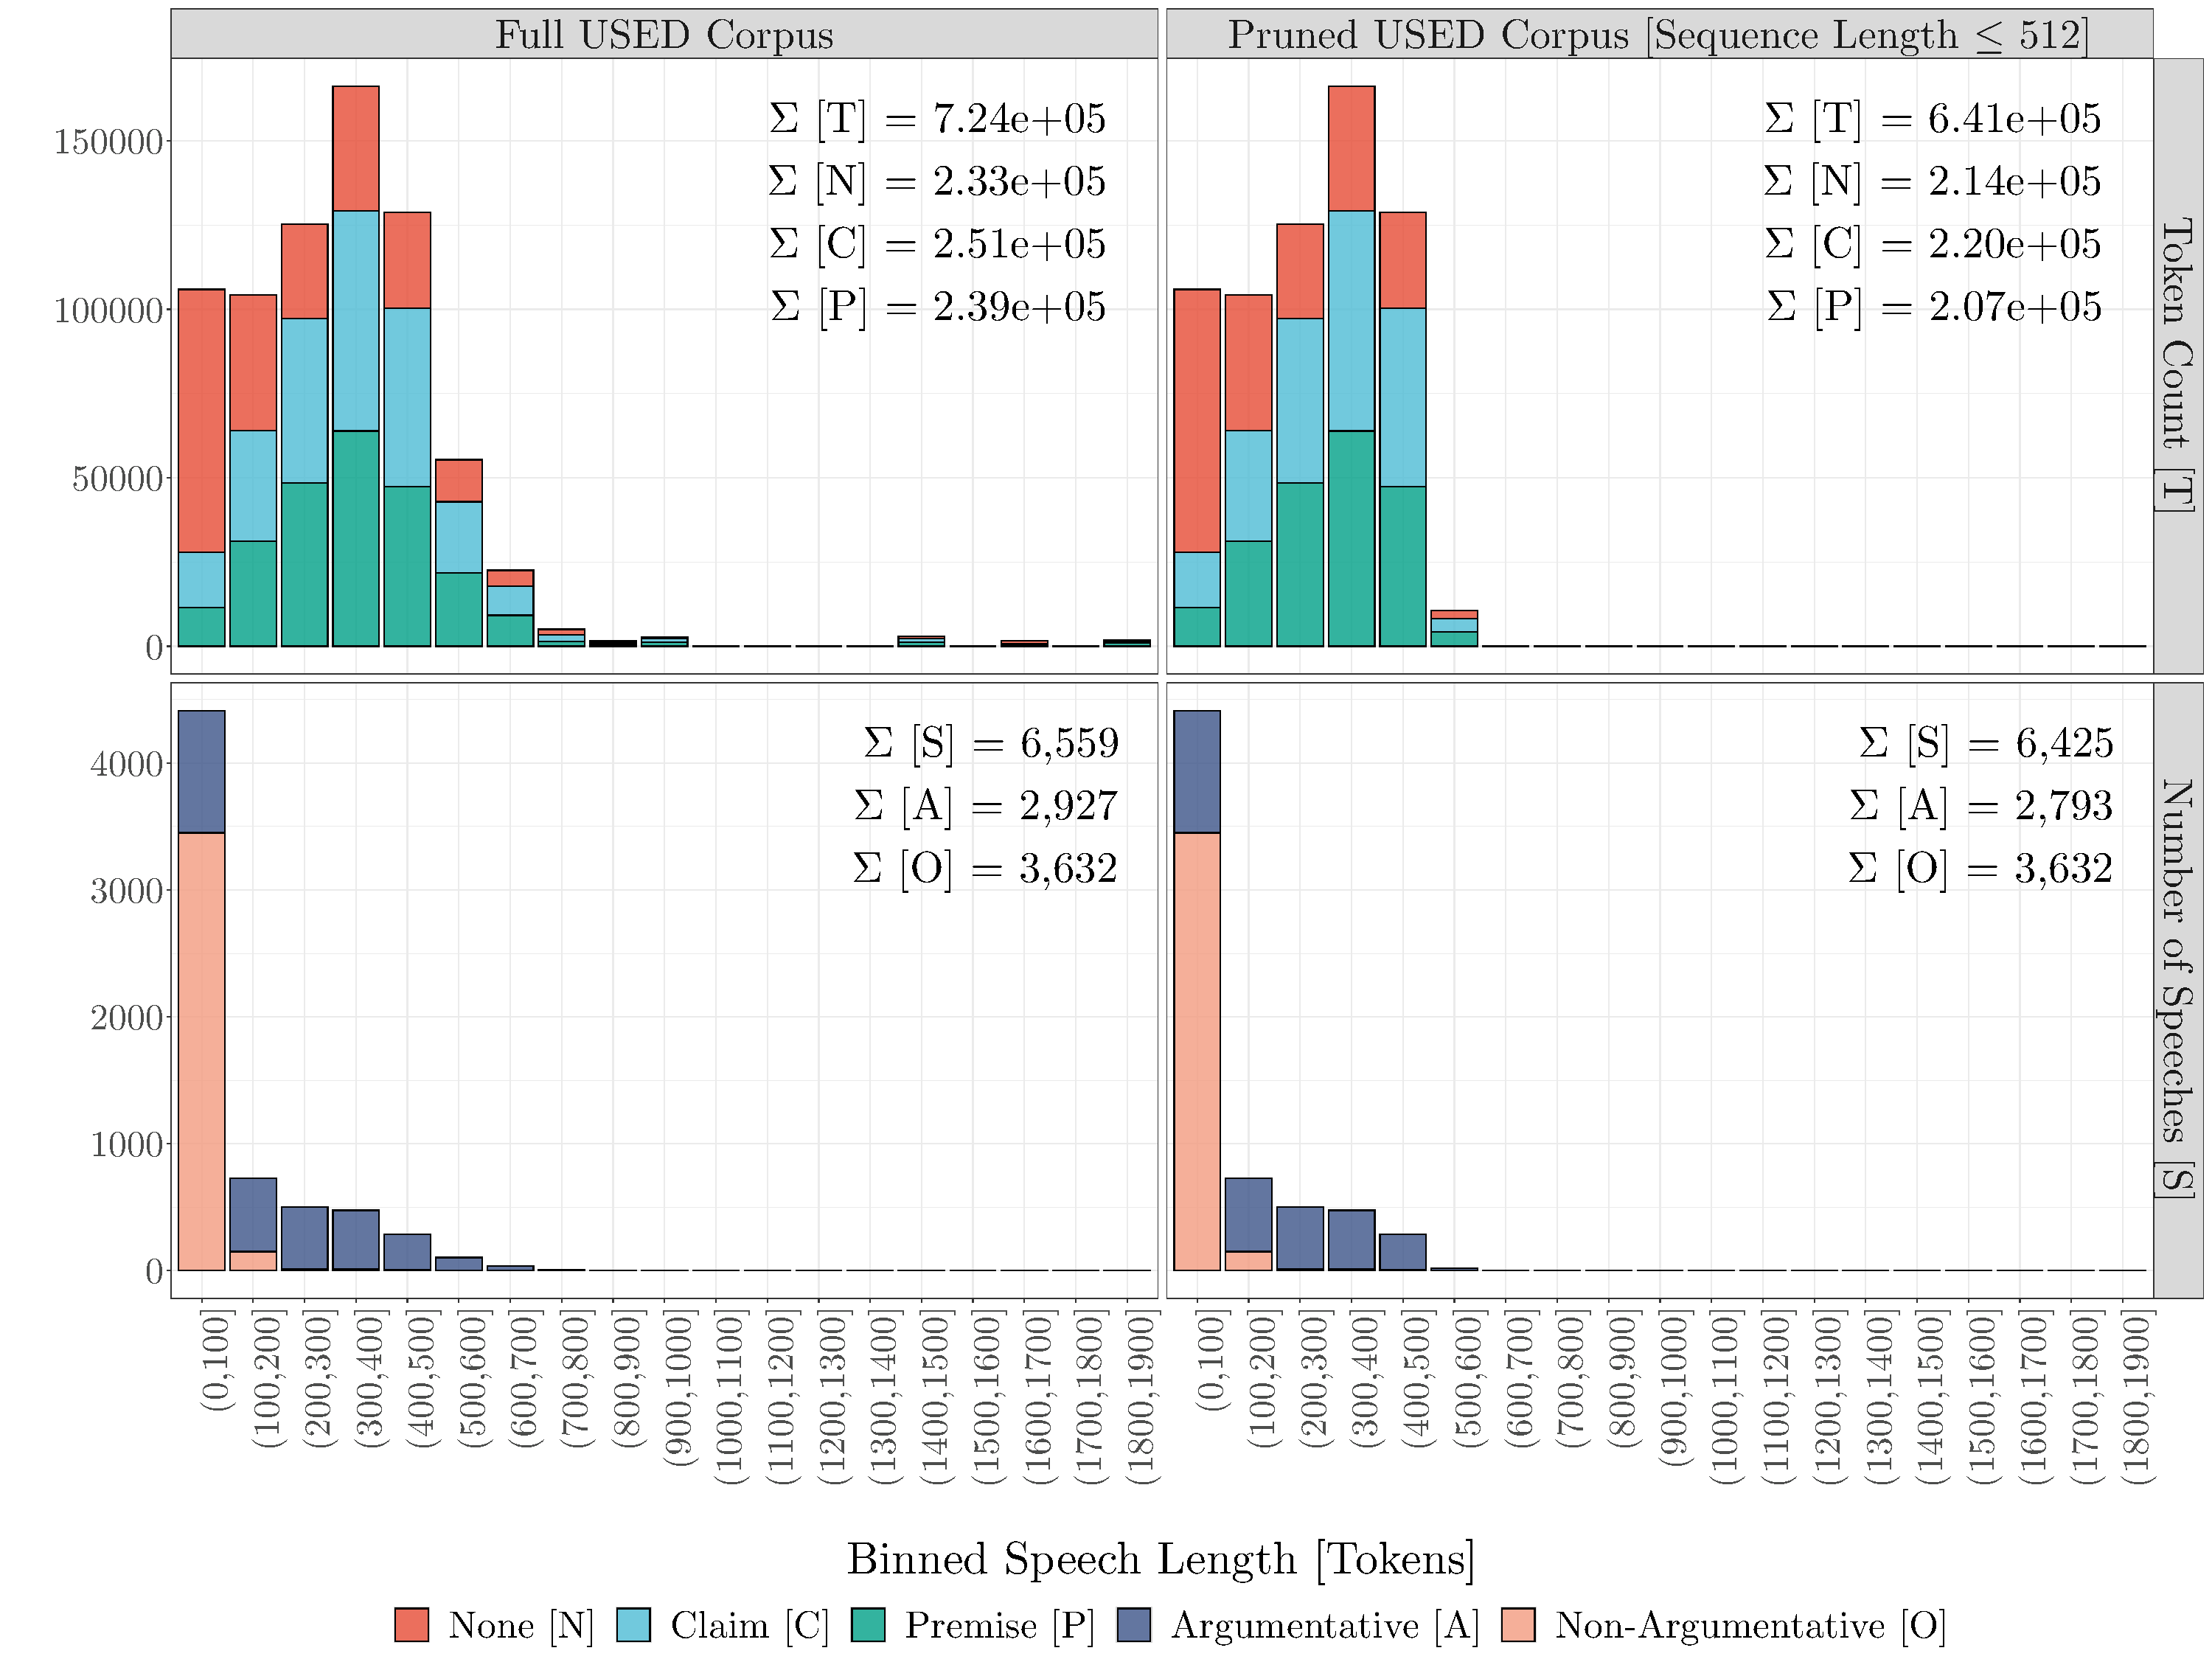
\includegraphics[trim={1.0cm 0cm 0cm 0cm},clip,width=\textwidth]{img/token_dist_US_length_combined.pdf}
    \caption{Full USED corpus (left-column) and pruned USED corpus (right-column) by binned speech length with token count (top-row) and number of speeches (bottom-row)}
    \label{used_distribution_combined}
\end{figure}

As mentioned in section \ref{corpora}, we decided that the USED corpus would be the best choice for us to train an argumentation classifier. Regarding corpus-specific ADUs, \citet{haddadan-etal-2019-yes}, the authors of the USED corpus, define a claim (in the political domain) as \textit{``a policy advocated by a party or a candidate to be undertaken which needs to be justified in order to be accepted by the audience."} Similarly, they define a premise as an \textit{``assertion made by the debaters for supporting their claims (i.e., reasons or justifications)."}

The USED corpus is annotated at a character-span level, with spans being annotated either as claims or premises. It follows naturally that character spans that are not annotated can be considered as non-argumentative text. Furthermore, the USED corpus also has been annotated for linkages between argumentative spans. This typically comes in the form of $N$ consecutive premises being recorded after a claim; which indicate that those $N$ premises belong to the preceding claim. Linkage types, such as attack or support relations, are not annotated in this corpus.

As mentioned in section \ref{models}, we would like to conduct argumentation mining using a bottom-up approach by using sequence tagging; since this process would also lend itself to quick application on the UNSC corpus. Given the time and resource restrictions in this study, we decided to focus solely on classifying tokens into argumentation candidates; such as claims, premises or neither. We omit the task of linking spans from claims and premises and instead recommend this task for further studies.

It is also worth noting that \citet{haddadan-etal-2019-yes} performed a similar task as ours on the USED corpus. However, they trained a classifier to identify argumentative sentences and argumentative sentence types. Performing such a task at a sentence-level removes many of the fine-grained character spans which do not necessarily span entire sentences. In fact, multiple character spans can be included within a sentence. As a result, we will be unable to compare our results directly with theirs since we perform a more fine-grained token-level classification task.

\subsubsection{Data Preprocessing}

\begin{figure}[b!]
    \centering
    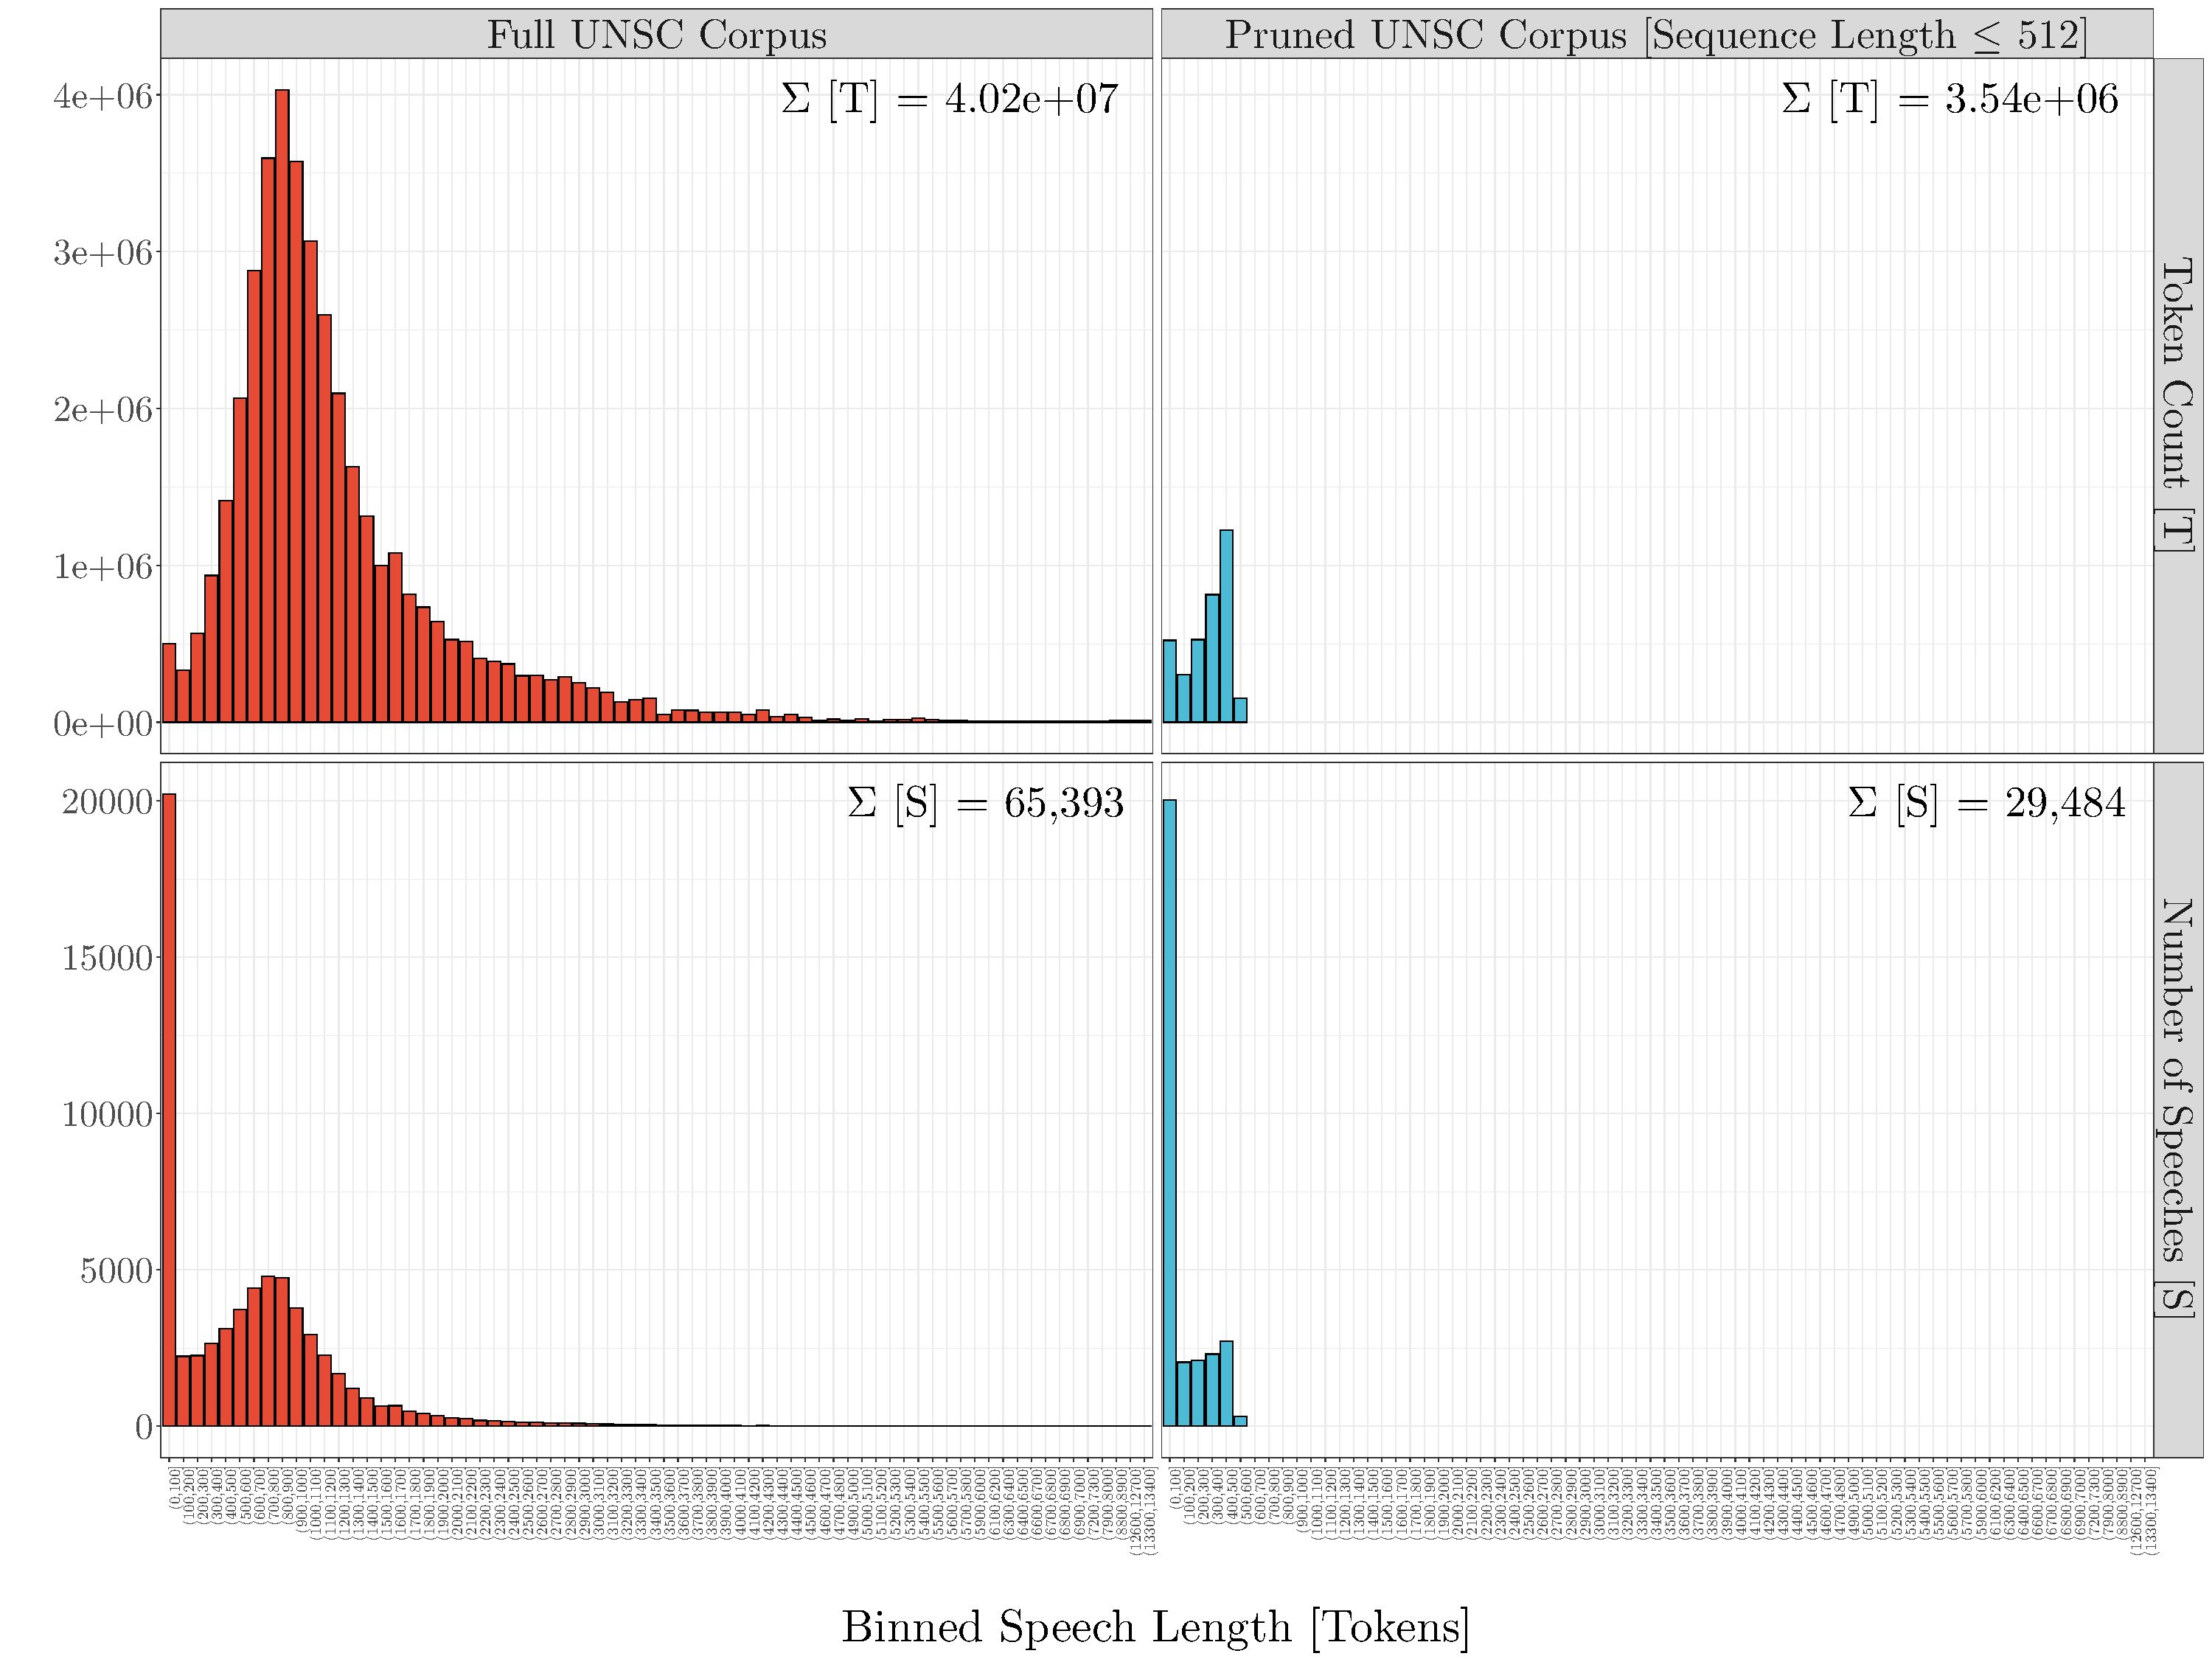
\includegraphics[trim={1.0cm 0cm 0cm 0cm},clip,width=\textwidth]{img/token_dist_UNSC_length_combined.pdf}
    \caption{Full UNSC corpus (left-column) and pruned UNSC corpus (right-column) by binned speech length with token count (top-row) and number of speeches (bottom-row)}
    \label{unsc_distribution_combined}
\end{figure}

Following a similar approach from \citet{eger2017neural}, we start by preparing the USED corpus for a sequence tagging task. Firstly, we converted character span annotations in the USED corpus to token-level annotations. Each token in the USED corpus gets mapped to one of three labels; specifically the ``None" (N), ``Claim" (C) or ``Premise" (P) label. Speeches that had at least one of either C or P tokens are considered argumentative (A), while speeches containing only N tokens are considered non-argumentative (O). The left column of Figure \ref{used_distribution_combined} shows the distribution of these classes of tokens as well as the number of speeches/types in the full USED corpus. It is worth noting that we omit the Beginning-Inside-Outside (BIO) tagging scheme as recommended in \citet{eger2017neural}; to keep our methodology simple and prevent label imbalances in the already small USED corpus. We also observe that sequences longer than 100 tokens tend to be more argumentative or have more C and P labels, indicating that longer sequences are of greater interest for argumentation mining in the USED corpus.

After mapping tokens to the aforementioned argumentation classes, we attempt to remove USED corpus-specific bias. In particular, we remove the initial token(s) in each speech where the identity of the person giving the speech is stated. Next, we use the SPM model to segment words into lowercased subwords; in accordance with the pre-packaged uncased ALBERT tokenizer. Finally we add BERT's special tokens; specifically a \texttt{[CLS]} and \texttt{[SEP]} token at the start and end of the sequence respectively. As mentioned in \ref{bert}, this process increases the token lengths of speeches; with some speeches exceeding the maximum sequence length of 512 tokens. To address this, we prune the USED corpus and remove sequences longer than 512 tokens. The effect of this pruning process can be seen in the right column of Figure \ref{used_distribution_combined}, with a minimal loss of 11$\%$ of tokens and 2$\%$ of speeches in the USED corpus.

The same data preprocessing procedure (naturally minus argumentation labelling) is then performed on the UNSC corpus to ensure that both these corpora can be treated similarly by the argumentation classifier model. For domain debiasing in the UNSC corpus, we also remove initial tokens which state the identity of the speaker. Figure \ref{unsc_distribution_combined} shows the effect of pruning on the UNSC corpus, with a much greater loss of 91$\%$ of tokens and 55$\%$ of speeches. Unfortunately, this is a necessary measure and is one of the major limitations of using the ALBERT model for such long sequences.

Finally, after pruning the corpora and having a clean set of input sequences, we insert BERT's \texttt{<pad>} tokens to cap up all sequences to 512 tokens, as this is necessary for the static computation graph that was implemented in our code. For evaluation purposes, we randomly split the USED corpus into \{training $\cup$ validation\} and test sets with a 70:30 ratio. We then split the \{training $\cup$ validation\} set into training and validation sets with a 85:15 ratio.

\subsubsection{Model Fine-Tuning and Evaluation}
\label{fine_tune}

\begin{table}[b]
	\centering
	\small
	\setlength{\tabcolsep}{0.5em}
	\def\arraystretch{1.1}
	\begin{threeparttable}
		\begin{tabular}{L{0.19\linewidth} p{0.52\linewidth} L{0.01\linewidth} L{0.17\linewidth}}
			\toprule[0.25mm]
			Model & Description && Parameters \\
			\midrule[0.35mm]
			TD$\_$Dense & 5 stacked time-distributed dense layers on top of the ALBERT model; with Rectified Linear Unit (ReLU) and softmax activations && 11,659,334 \\\\[-5pt]
			1D$\_$CNN & 5 stacked 1-dimensional convolutional layers on top of the ALBERT model; with ReLU and softmax activations && 12,790,598 \\\\[-5pt]
			Stacked$\_$LSTM & 3 stacked Long Short-Term Memory (LSTM) layers on top of the ALBERT model; with ReLU and softmax activations && 14,709,446 \\
			\bottomrule[0.25mm]
		\end{tabular}
		\caption{Tabular summary of three end-to-end ALBERT model types with custom decoders}
		\label{table_arg_train_models}
	\end{threeparttable}
\end{table}

As mentioned in section \ref{albert}, we decided that the ALBERT language model would be a good choice for us to fine-tune for our argumentation mining task. With the USED and UNSC corpora preprocessed, we needed to finalize the ALBERT model for fine-tuning. Out of the box, the ALBERT model is an encoder model. In order to use it for a supervised argumentation sequence tagging task, we would need to extend ALBERT with custom decoders such that the output of the model would be in the appropriate dimensions. Table \ref{table_arg_train_models} provides a summary of three models that we fine-tuned in this study.

For the fine-tuning process, we assume a warmup-cooldown learning rate profile, where the learning rate rises linearly over the warmup epochs until a maximum learning rate and then exponentially decays till an end learning rate at a fixed upper limit of 100 epochs. We utilize the Adam optimizer for fine-tuning all our models. To determine the best model and corresponding hyperparameters, we conduct a grid-search over model-type, warmup-epochs, maximum learning rate and end learning rate.

It is worth noting here that we fix our fine-tuning batch-size at 10 samples to prevent GPU out-of-memory (OOM) issues. This is mainly because the ALBERT model has a high memory consumption that is exacerbated by its $O(N^2)$ space complexity due to the self-attention mechanism, where $N$ is the input sequence length. Because of this, our model fine-tuning process suffers from noisy gradients. We recommend solutions for this issue in section \ref{reco} of our study.

For the evaluation process, we employ early stopping with a patience value of 5 epochs; measuring the cross-entropy loss on the validation set. At the end of fine-tuning each model, we compute the model's performance on the test dataset and record its Macro-F$_1$ score over N, C and P argument labels. The model with the best test F$_1$ score is deemed as the best performing model. We provide our best fine-tuned model in our GitHub repository\footnotemark[\value{footnote}].

For all the aforementioned processes, we utilized the \texttt{bert-for-tf2} python library, which is written using Google's \texttt{TensorFlow} API. In terms of hardware, we utilized a single NVIDIA GeForce GTX 1080 Ti GPU with 12 GB RAM provided by the University of Potsdam.

\subsubsection{Prediction on UNSC}

After following the aforementioned fine-tuning and model evaluation process, we arrive at our best performing model. In order to use this model to predict argumentation token-level argumentation candidates in the UNSC corpus, we simply pipe the preprocessed UNSC corpus into the model and acquire the model's outputs.

Due to the static configuration of our model, the output will have a sequence length of 512 tokens. We then remove the output sequence positons which correspond to the BERT \texttt{[CLS]}, \texttt{[SEP]} and \texttt{<pad>} special tokens; leaving behind only the important sub-word tokens that have been classified into N, C or P argumentation candidates. As a final product, we compile our UNSC predictions into a human-readable \texttt{json} file in our GitHub repository\footnotemark[\value{footnote}], which maps UNSC speech IDs to token-level argumentation predictions.
\section{Results}
\label{results}

\subsection{Sentiment Analysis}
Given the abundance of UNSC session data available, we decided to narrow the scope of our analysis using different approaches. First, we examined to most popular topics in order the determine whether trends can be seen. Secondly, we took a look at the big picture and analyzed the sentiment development for each country in the time frame 1995-2017. Finally, we decided to analyze the core nations of the UNSC, since the corpus provides consistent data for the entire time frame. In addition to this, we analyzed the sentiment in Iraq War related sessions. 
\subsubsection{Topics}
In order to get a grasp of the contents of the sessions, we examined the most common topics for the provided time frame and each year respectively. Figure \ref{common_1} visualizes the 20 most common topics for the UNSC speeches. It can be observed that there is no uniform naming convention for the topics. The most discussed topic is \textit{Middle East situation, including the Palestinian question} and the topic on rank six is \textit{The situation in the Middle East, including the Palestinian question}. In other analyses, the topic name \textit{The situation in the Middle East} occurs as well. It can be assumed that the different topic names refer to one and the same topic.  
Interestingly, the Middle East topic occurs in the most discussed topics for the first time in 2000 and remains in the top 5 most discussed topics for the entirety of 2000-2017, despite the inconsistent naming convention.

\begin{figure}[t]
  \centering
  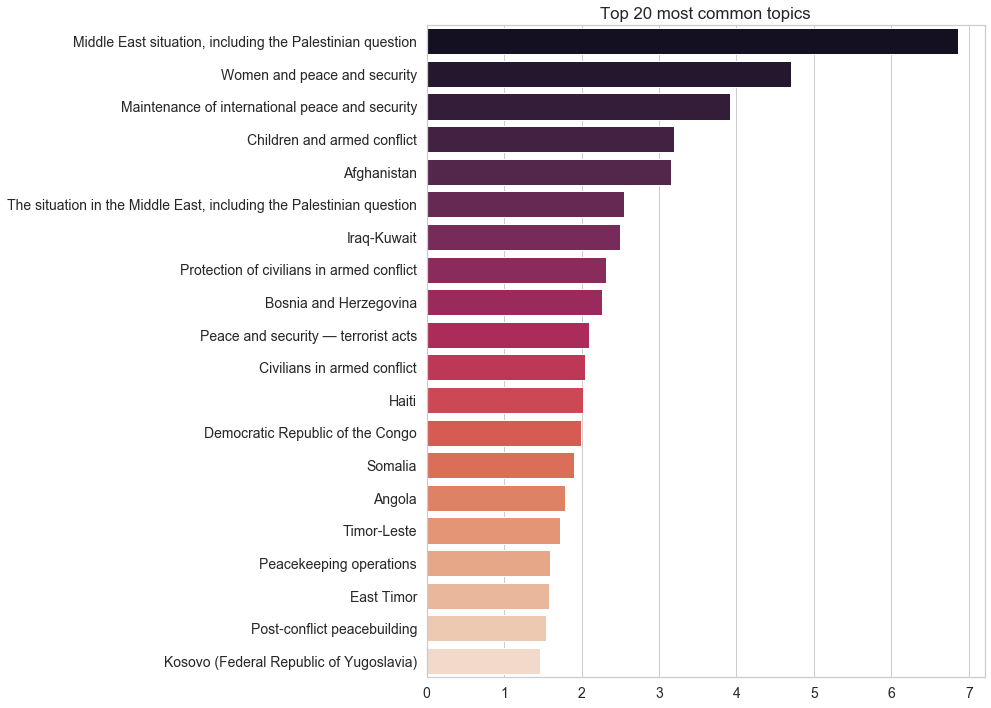
\includegraphics[width=14.5cm]{img/20most_common_topics.png}
  \caption{The 20 most common topics in the UNSC}
  \label{common_1}
\end{figure}%

A shift in topics can be observed after the year 2001. The most common topics diverged from humanitarian ones (e.g. Africa, Angola, East Timor) to more fundamental ones (e.g. Peace and Security - terrorist acts, Women and Peace and Security, Post-conflict peacebuilding). Figure \ref{common_2} and Figure \ref{common_3} visualize the differences in topics for 1996 and 2003. 



\begin{figure}[t]
  \centering
  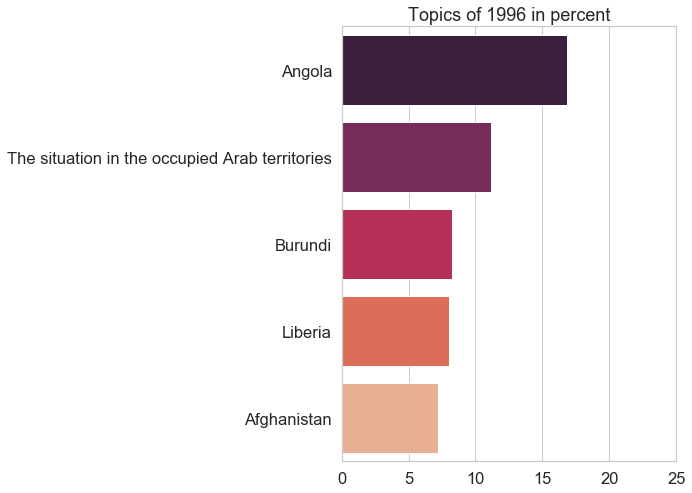
\includegraphics[width=12cm]{img/1996_most_common_topics.png}
  \caption{Most common topics in 1996}
  \label{common_2}
  
\end{figure}%
\begin{figure}[t]
  \centering
  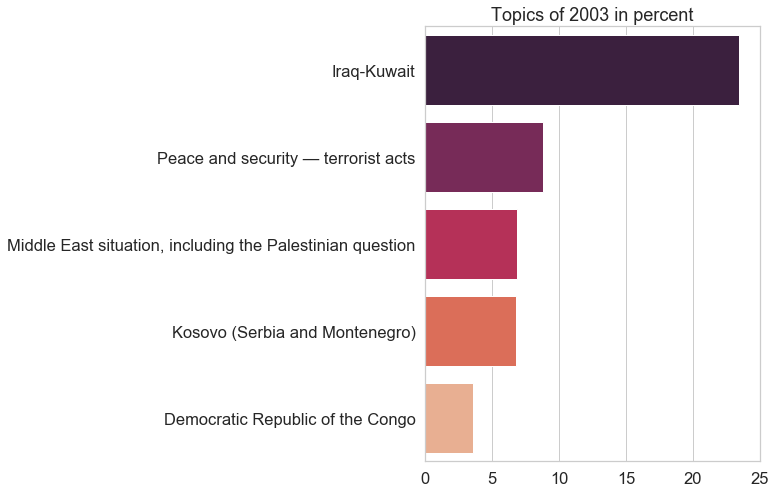
\includegraphics[width=12cm]{img/2003_most_common_topics.png}
  \caption{Most common topics in 2003}
  \label{common_3}
\end{figure}%

\subsubsection{Sentiment in the UNSC}
The sentiment analysis in the UNSC was conducted on 182 individual members of the council, sovereign nations and independent members were included. As could be expected, the participation varies among the members. For some countries, only scarce data is available, e.g. Belize, which only took part in four years of council meetings. Other countries attended the council meetings more frequently, with many countries appearing in all 23 years of the analysis. It is also worth noting that some countries' names changed over time, e.g. Zaire, which is now known as Democratic Republic of the Congo, and some countries do not exist anymore, e.g. the former Yugoslavia.

\begin{figure}[t!]
    \centering
    \begin{minipage}{0.47\textwidth}
        \centering
        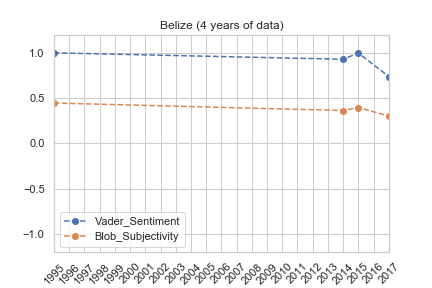
\includegraphics[width=1.1\textwidth]{img/Belize_average.png} % first figure itself
        \caption{Sentiment Analysis for Belize}
        \label{belize}
    \end{minipage}\hfill
    \begin{minipage}{0.47\textwidth}
        \centering
        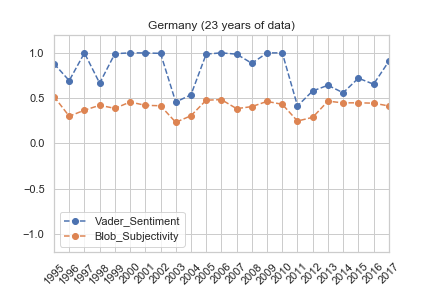
\includegraphics[width=1.1\textwidth]{img/Germany_average.png} % second figure itself
        \caption{Sentiment Analysis for Germany}
        \label{germany}
    \end{minipage}
\end{figure}

The visualizations of the sentiment and subjectivity analysis for Belize (Figure \ref{belize}) and Germany (Figure \ref{germany}) suggest a correlation between sentiment and subjectivity scores. A higher polarity in sentiment occurs with an increase in subjectivity in the analysis for Belize, while the lower sentiment scores come with an increase in objectivity for Germany. For Germany, especially the year 2003 stands out. 2003 was the beginning of the Iraq War, of which Germany was a vocal opponent \citep{germiraq}.

\subsubsection{Sentiment in the Core Nations}
After completing the topic and sentiment analysis for the UNSC, we decided to narrow the scope of our investigations. A comparative and exploratory analysis yields the best results if the data is not skewed, i.e. equally distributed. For this reason, we laid our focus for the sentiment analysis on the core nations of the UNSC, which are the People's Republic of China, the French Republic, the Russian Federation, the United Kingdom of Great Britain and Northern Ireland, and the United States of America.

These core nation are granted a permanent member status of the council as per the Charter of the United Nations, a treaty from 1945\footnote{\href{https://www.un.org/en/charter-united-nations/}{https://www.un.org/en/charter-united-nations/}}. A permanent membership entails a \textit{Power of Veto}, which allows voting against UNSC resolutions and thus preventing their adoption. 
The core nations were a suitable subject for our analysis since they participated in most of the UNSC meetings. Not only could we rely on data for every year provided in the corpus, we could also assume that important resolutions would be included in the analysis.

\begin{figure}[t]
  \centering
  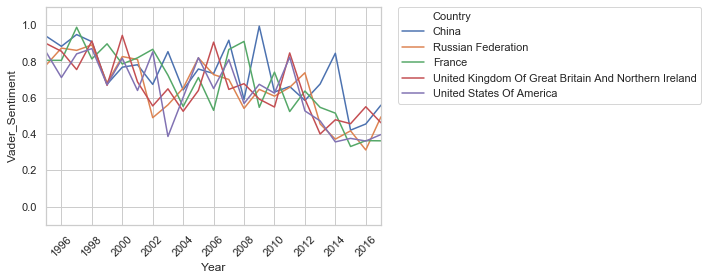
\includegraphics[width=14cm]{img/over_time_Vader_Sentiment.png}
  \caption{Sentiment development in the UNSC core nations}
  \label{fig:vadercore}
\end{figure}%

The sentiment analysis for the UNSC core nations shows a general downward trend in sentiment polarity (Figure \ref{fig:vadercore}). Significant negative peaks were revealed for historical events, e.g. the year 2002 for the Russian Federation and the year 2003 for the United States of America, both possibly related to the imminent Iraq War.

\begin{figure}[b]
  \centering
  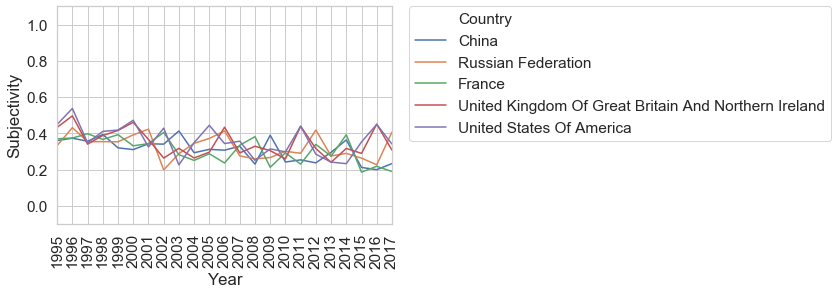
\includegraphics[width=14cm]{img/over_time_Blob_Subjectivityy.png}
  \caption{Subjectivity development in the UNSC core nations}
  \label{fig:subjcore}
\end{figure}%

The visualization of the subjectivity analysis (Figure  \ref{fig:subjcore}) shows a mostly consistent development of subjectivity in the core nations but suggests a slight downward trend, meaning a rise in objectivity, over the investigated time frame. This is consistent with the observation made in %link subsubsection sentiment in the unsc 
the sentiment analysis conducted on all members of the UNSC. The negative peaks in sentiment mentioned for Russia and the USA, 2002 and 2003 respectively, also appear as negative, more objective, peaks in the subjectivity analysis.

\subsubsection{Sentiment regarding the Iraq War}
%%% should this go in background info??
As the topic for an in-depth analysis, we chose the Iraq War. Until today, the Iraq War and the UNSC's involvement in it is a highly polarizing topic. Kofi Annan, the United Nations Secretary-General, stated that ``the US-led invasion of Iraq was an illegal act that contravened the UN charter" \citep{bbciraq}.
The possibility of an invasion arose from the speculation that Iraq was in possession of weapons of mass destruction, after the UNSC council unanimously adopted Resolution 1441 which gave Iraq "a final opportunity to comply with its disarmament obligations" \citep{resolution1441}.
This issue also divided the core nations of the Security Council.

The United States of America were a strong proponent of pursuing military action against Iraq, with or without approval of the UNSC \citep{usairaq}. The United Kingdom supported this policy.
France on the other hand was strictly against the war. The former president Jacques Chirac went as far as saying he would make use of his veto right to prevent the adoption of a resolution that would allow for a military intervention in Iraq \citep{nyt}.
China was more reserved in taking a position on this matter, yet stated that their position was ``extremely close to that of France" \citep{cnn}. Russia also did not have a consistent policy on this matter, first being against an invasion and later on becoming more neutral and even approving of the USA's plans \citep{russiairaq}.
On March 19, 2003, an U.S.-led coalition invaded Iraq.

\vspace{-5pt}
\paragraph{General Sentiment}
In order to examine the general sentiment of the core nations regarding the Iraq War, we extracted all speeches with a topic labelled ``Iraq" or ``Iraq-Kuwait". 

\begin{figure}[H]
    \centering
    \begin{minipage}{0.47\textwidth}
        \centering
        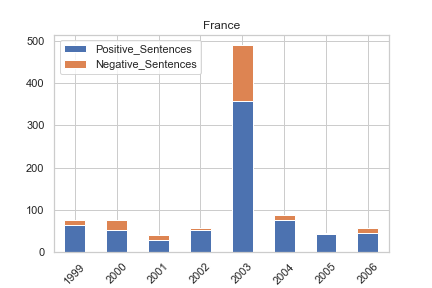
\includegraphics[width=1.1\textwidth]{iraq_scores_France.png} % first figure itself
        \caption{Polarity distribution regarding \\ Iraq for France}
        \label{iraqfr}
    \end{minipage}\hfill
    \begin{minipage}{0.47\textwidth}
        \centering
        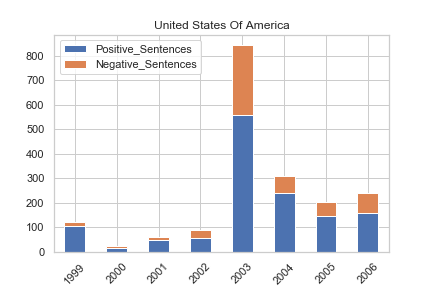
\includegraphics[width=1.1\textwidth]{iraq_scores_United States Of America.png} % second figure itself
        \caption{Polarity distribution regarding \\ Iraq for the USA}
        \label{iraqusa}
    \end{minipage}
\end{figure}

\begin{figure}[H]
    \centering
    \begin{minipage}{0.47\textwidth}
        \centering
        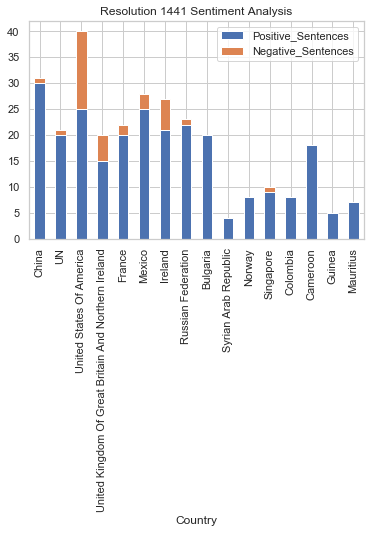
\includegraphics[height=1.3\textwidth]{Resolution 1441_sentiment.png} % first figure itself
        \caption{Sentiment regarding Resolution \\ 1441}
        \label{1441sent}
    \end{minipage}\hfill
    \begin{minipage}{0.47\textwidth}
        \centering
        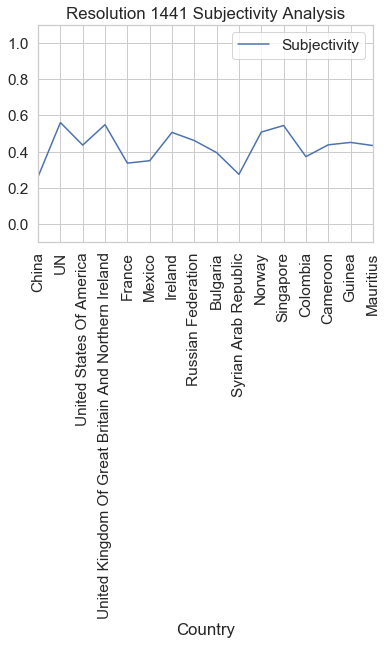
\includegraphics[height=1.3\textwidth]{Resolution 1441_subjectivity.png} % second figure itself
        \caption{Subjectivity regarding Resolution \\ 1441}
        \label{1441subj}
    \end{minipage}
\end{figure}

For presenting the results of the analysis, we chose two countries with opposing opinions on the invasion of Iraq, France (Figure \ref{iraqfr}) and the United States of America (Figure \ref{iraqusa}).
For both countries, the amount of sentences with polarity with regard to Iraq is the highest for the year 2003, due to the Iraq War. Before and after 2003, France contributed on average less than 100 sentences on this topic, an increase after 2003 cannot be observed. This is different for the USA. Before 2003, the analysis reveals years were the country contributed fewer sentences than France, with 1999 being the the year with the most contributions and 2000 being the year with the fewest. After 2003, the USA consistently contributed more than 200 negative and positive sentences per year, which is significantly more than all other core nations.

In 2003, the representatives of the USA contributed more than 800 sentences with polarity, with roughly a third of them being negative. 
For France, the country representatives uttered almost 500 relevant sentences with roughly a quarter of them being negative.

\paragraph{In-Depth: Iraq War related Resolutions}
In order to give a better insight into Iraq War related resolutions, we focused on two sessions that were highly significant in the year leading to the invasion of Iraq. First, we examined Resolution 1441, a resolution that was adopted in the 4644th session of the UNSC on 18 November 2002. As mentioned before, it granted Iraq "a final opportunity to comply with its disarmament obligations" \citep{resolution1441} and subsequently lead to the invasion of Iraq, after the country allegedly failed to comply with said disarmament obligations.

\begin{figure}[b!]
    \centering
    \begin{minipage}{0.45\textwidth}
        \centering
        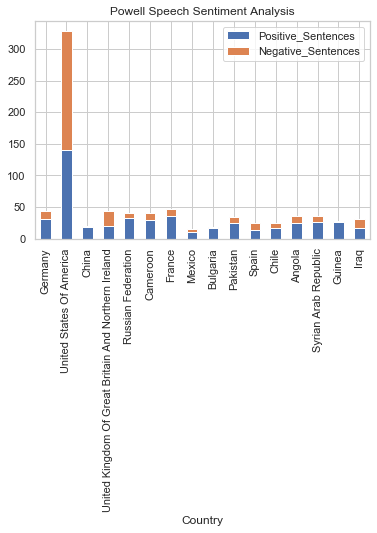
\includegraphics[height=1.3\textwidth]{Powell Speech_sentiment.png} % first figure itself
        \caption{Subjectivity regarding Powell's \\ speech}
        \label{powellsent}
    \end{minipage}\hfill
    \begin{minipage}{0.45\textwidth}
        \centering
        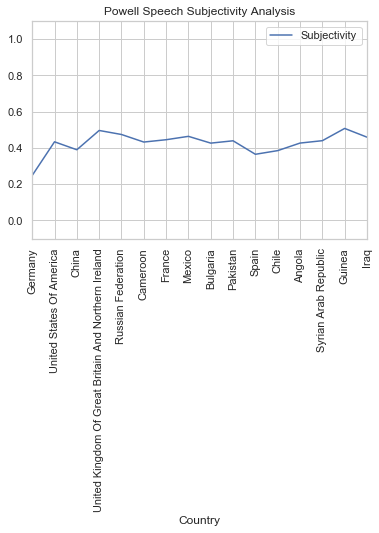
\includegraphics[height=1.3\textwidth]{Powell Speech_subjectivity.png} % second figure itself
        \caption{Subjectivity regarding Powell's \\ speech}
        \label{powellsubj}
    \end{minipage}
\end{figure}

In the sentiment analysis visualizations (Figure \ref{1441sent}) it can be observed that the USA contributed more to the session than the other countries. The highest negative/positive sentence ratio can be observed for the USA and the UK, along with Ireland. While the former two countries were in favor of the ``consequences" announced in Resolution 1441, Ireland had a neutral stance on this policy.

The subjectivity scores (Figure \ref{1441subj}) are roughly distributed between 0.3 and 0.6, which indicates a varying level of objectivity with regard to this resolution.

Secondly, we analyzed session 4701 from February 5, 2003 in which United States Secretary of State Colin Powell discussed the urgency of attacking Iraq as it was allegedly in possession of a mobile production facility for biological weapons \citep{cia}. This speech was controversial in the UNSC and later on it became evident that it was not based on facts but solely on speculations. Neither the USA nor the UK were able to provide evidence for their claims \citep{iraqev}. 
Powell himself said later: ``I regret it. I will always regret it. It was a terrible mistake on all our parts and on the intelligence community." \citep{powell}.

It can be observed that Powell (i.e. the USA) uses a very negative vocabulary (Figure \ref{powellsent}). He contributes significantly more than the other participants (~330 sentences) and more than half of his speech has a negative polarity. A similar ratio of positive to negative sentences can be observed for the UK, although they do not participate more than the other countries involved. This aligns with the previously discussed division of the UNSC regarding the invasion of Iraq and the fact that the USA and the UK were proponents of this approach.

The subjectivity scores (Figure \ref{powellsubj}) concerning the Powell session seem rather homogeneous in comparison to the ones regarding Resolution 1441, except for Germany, which has an unusually low subjectivity score. As discussed before, Germany was a strong opponent of the Iraq War.

\subsection{Argumentation Mining}
\subsubsection{Model Fine-Tuning and Evaluation}

As mentioned in section \ref{fine_tune}, we fine-tuned three different model types using a grid-search technique. We ran the grid-search fine-tuning (or training) for 1.5 days on a single GPU, evaluating our results against the USED test set. We compared these models with a baseline majority-class classifier; which predicted all tokens in the test set as claim tokens which form the majority class.

\begin{table}[b!]
	\centering
	\small
	\setlength{\tabcolsep}{0.5em}
	\def\arraystretch{1.1}
	\begin{threeparttable}
		\begin{tabular}{L{0.20\linewidth} L{0.11\linewidth} L{0.10\linewidth} L{0.14\linewidth} L{0.14\linewidth} L{0.14\linewidth}}
			\toprule[0.25mm]
			Model & Training Epochs$^{\ddagger}$ & Test F$_1$ & Test F$_1$ [N] & Test F$_1$ [C] & Test F$_1$ [P] \\
			\midrule[0.35mm]
			Baseline$^{\dagger}$ & -- & 0.173 & 0.000 & 0.518 & 0.000  \\
			\textbf{TD$\_$Dense} & 17 & \textbf{0.693} & \textbf{0.763} & \textbf{0.689} & 0.627 \\
			1D$\_$CNN & 16 & 0.689  & 0.758 & 0.659 & \textbf{0.651} \\
			Stacked$\_$LSTM & 21 & 0.633 & 0.679 & 0.624 & 0.596 \\
			\bottomrule[0.25mm]
		\end{tabular}
	\begin{tablenotes}[flushleft]
      \scriptsize
      \item $^{\dagger}$Baseline model is a majority classifier for the C token, which has the highest frequency in the test set
      \item $^{\ddagger}$Training epochs include five extra patience epochs; best model was saved from the lowest validation loss epoch
    \end{tablenotes}
		\caption{Tabular summary of model performance on the USED test set; bold implies best performance for given category}
		\label{table_arg_model_performances}
	\end{threeparttable}
	
	\centering
	\small
	\setlength{\tabcolsep}{0.5em}
	\def\arraystretch{1.1}
	\begin{threeparttable}
		\begin{tabular}{L{0.17\linewidth} L{0.23\linewidth} L{0.15\linewidth} L{0.15\linewidth} L{0.15\linewidth}}
			\toprule[0.25mm]
			Statistic & Macro-Average & None [N] & Claim [C] & Premise [P] \\
			\midrule[0.35mm]
		    Precision & 0.703 & 0.826 & 0.633 & 0.651  \\
		    Recall & 0.691 & 0.710 & 0.757 & 0.605  \\
			\bottomrule[0.25mm]
		\end{tabular}
		\caption{Tabular summary of precision-recall statistics for TD$\_$Dense model on the test set}
		\label{table_arg_model_PR}
	\end{threeparttable}
\end{table}

Our final model results are summarized in Table \ref{table_arg_model_performances}. While the 1D$\_$CNN model performed best in classifying premise tokens, the TD$\_$Dense model performed best on the overall USED test set with a Macro-F$_1$ score of 69.3$\%$. Table \ref{table_arg_model_PR} shows the precision-recall scores for the TD$\_$Dense model on the USED test set. Overall, we can observe a higher performance for N tokens compared to C and P tokens; which is in some ways intuitive since N tokens aggregate together in non-argumentative speeches, while C and P tokens are distributed in tight spans within argumentative speeches. This might make the detection of C and P tokens more nuanced compared to the N tokens. Next, we can observe the performance of the TD$\_$Dense model with respect to training epochs in Figure \ref{model_performance}. This figure further emphasizes the point that fine-tuning is fast and computationally inexpensive; with the lowest validation cross-entropy loss being achieved in just 12 training epochs.

\begin{figure}[t!]
    \centering
    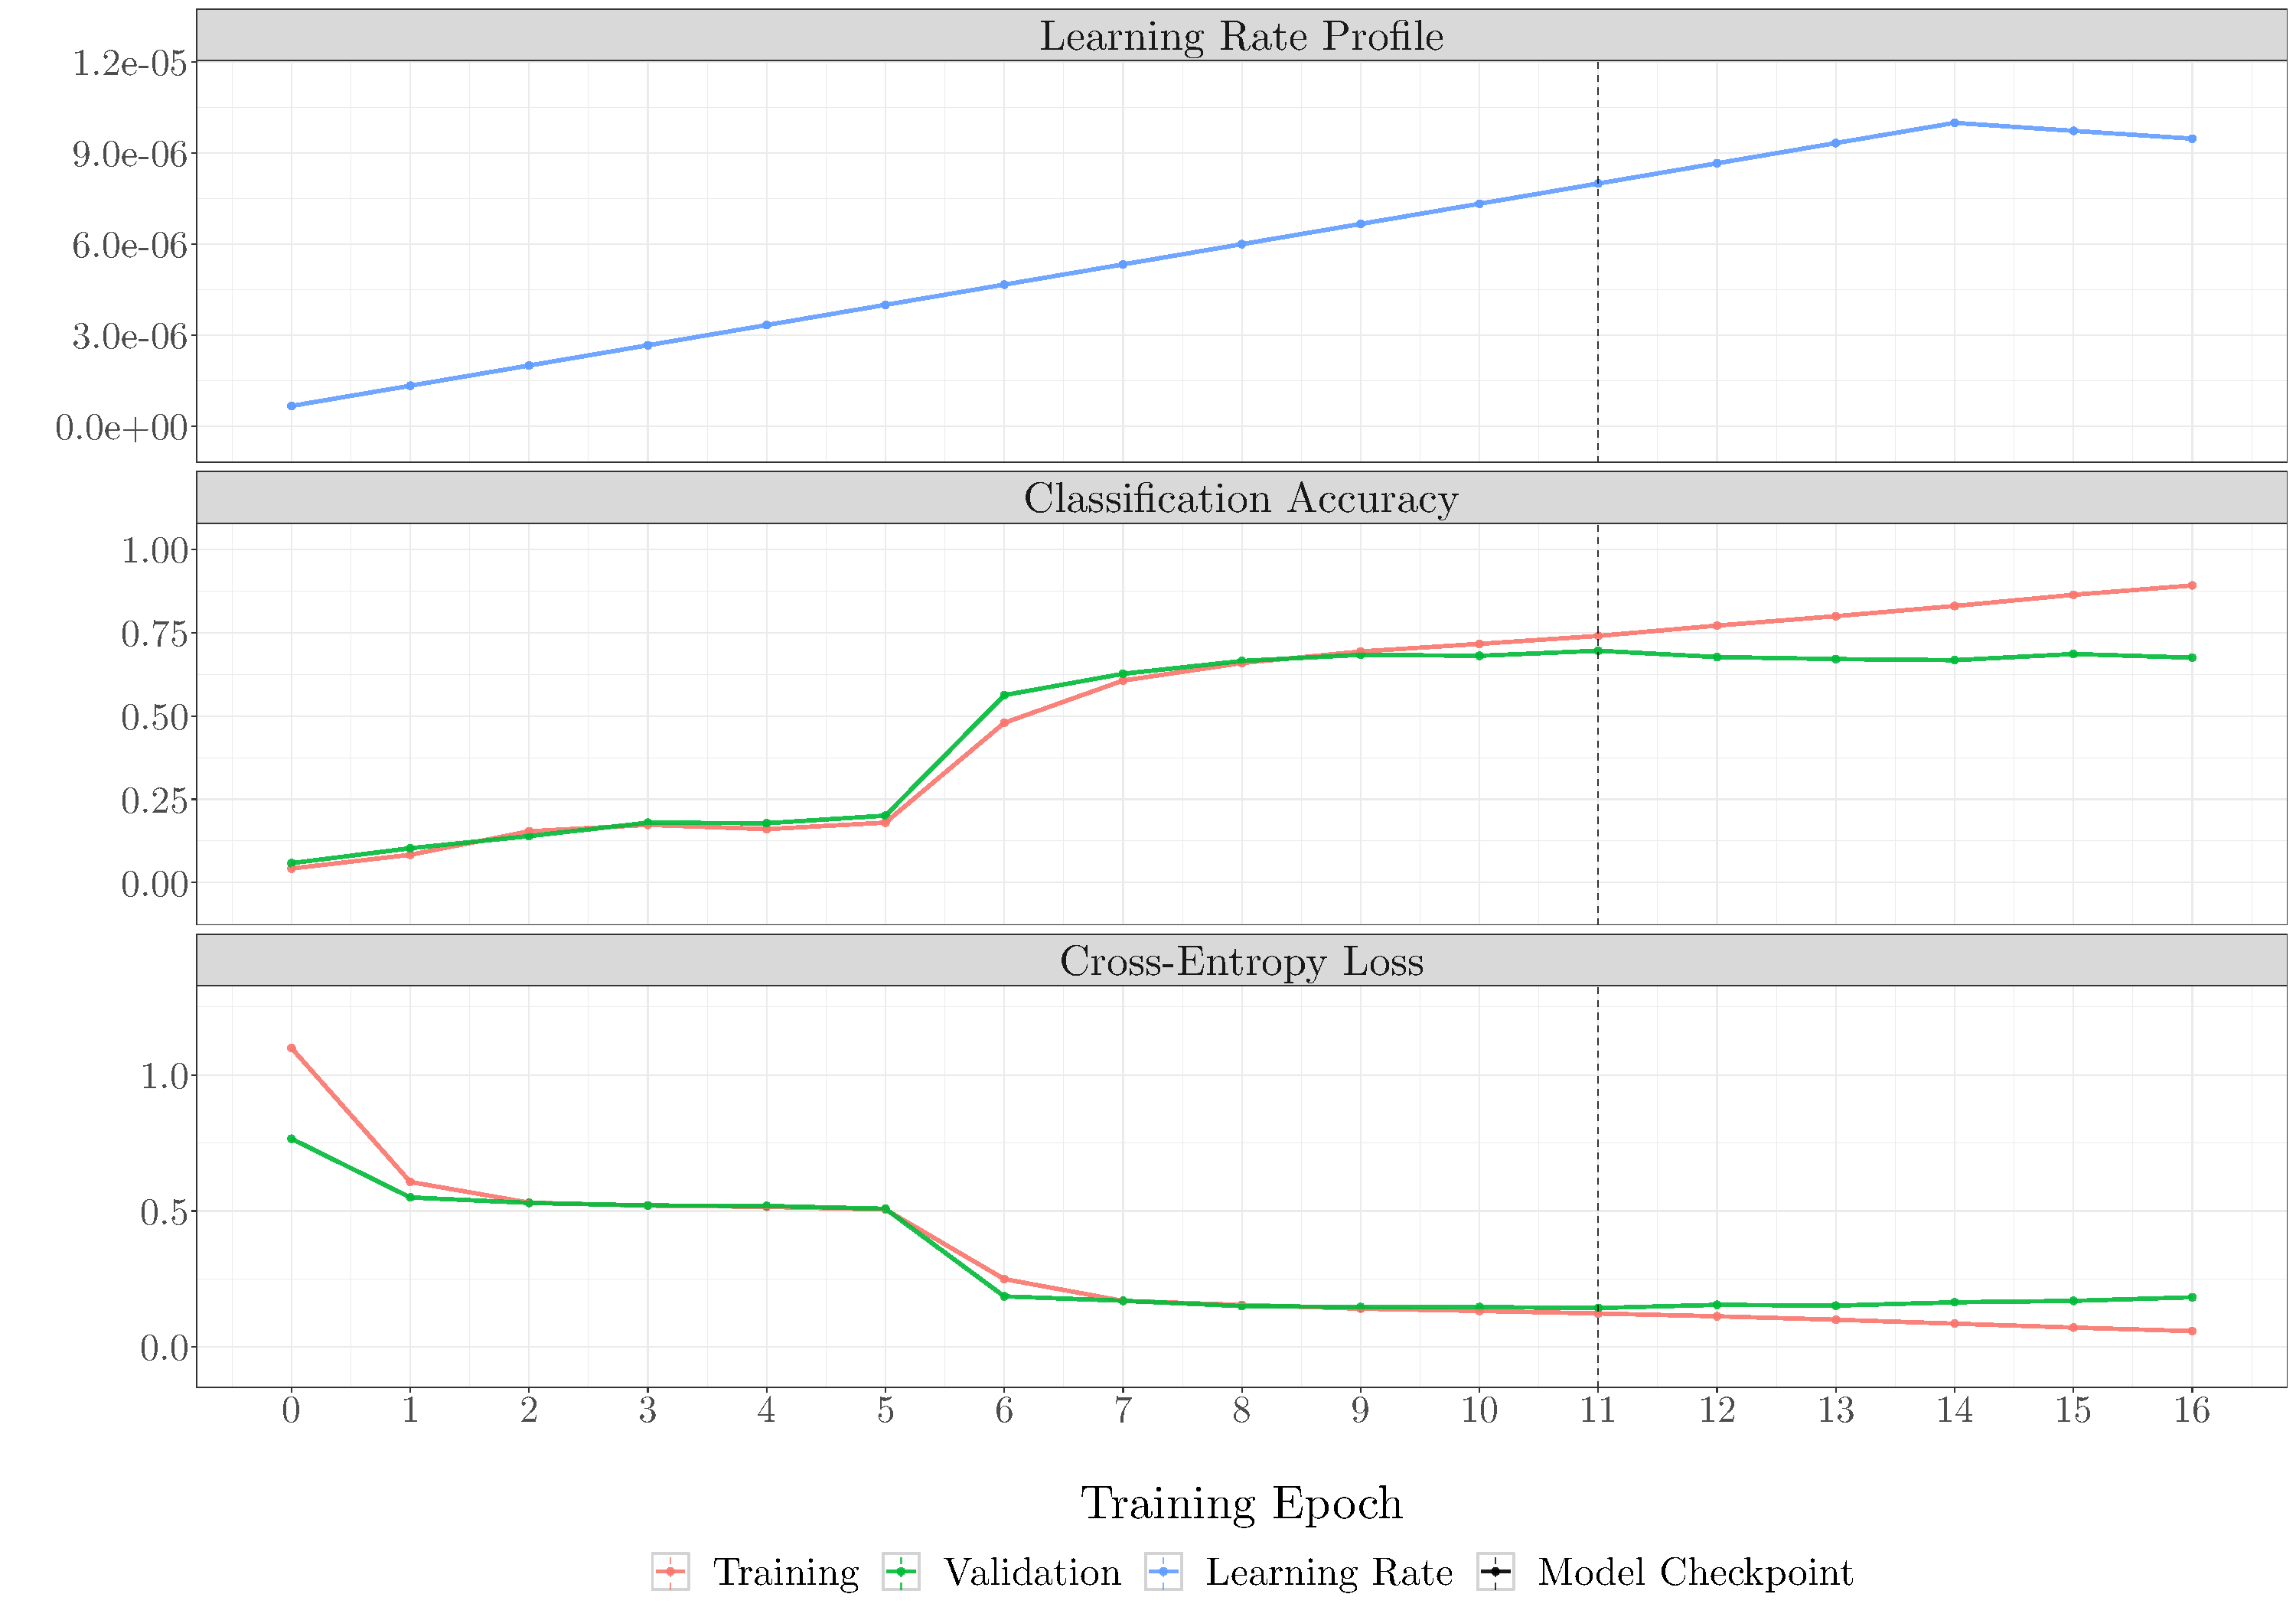
\includegraphics[trim={1.0cm 0cm 0cm 0cm},clip,width=\textwidth]{img/model_training_evolution.pdf}
    \caption{TD$\_$Dense model performance summary statistics by training epochs; black vertical line demarcates the 12th training epoch where validation cross-entropy loss was minimized}
    \label{model_performance}
\end{figure}

\subsubsection{Prediction on UNSC}

After identifying the best model as the TD$\_$Dense model, we then used this model to predict token-level argumentation labels of the preprocessed (pruned) UNSC corpus. Figure \ref{unsc_pred} shows the token distribution of the predictions of our best classifier on the UNSC corpus. Similar to the token distributions in the USED corpus as shown in Figure \ref{used_distribution_combined}, we observe that the proportions of claim and premise tokens, as well as argumentative speeches, increase as the speech sequence lengths increase. However, unlike the USED corpus' balanced token/speech distributions in Figure \ref{used_distribution_combined}; our fine-tuned model's predictions appear to show a strong skew towards N tokens and non-argumentative speeches.

There could be many reasons for this; one of which could be a bias towards more informal argumentation structures in the USED corpus which might conflict with the formalized argumentation structures in the USED corpus. In section \ref{manual_semantic}, we will perform some manual semantic analyses of positive and negative UNSC predictions to sample, albeit in an extremely limited manner, performance on the UNSC corpus. 

\begin{figure}[t!]
    \centering
    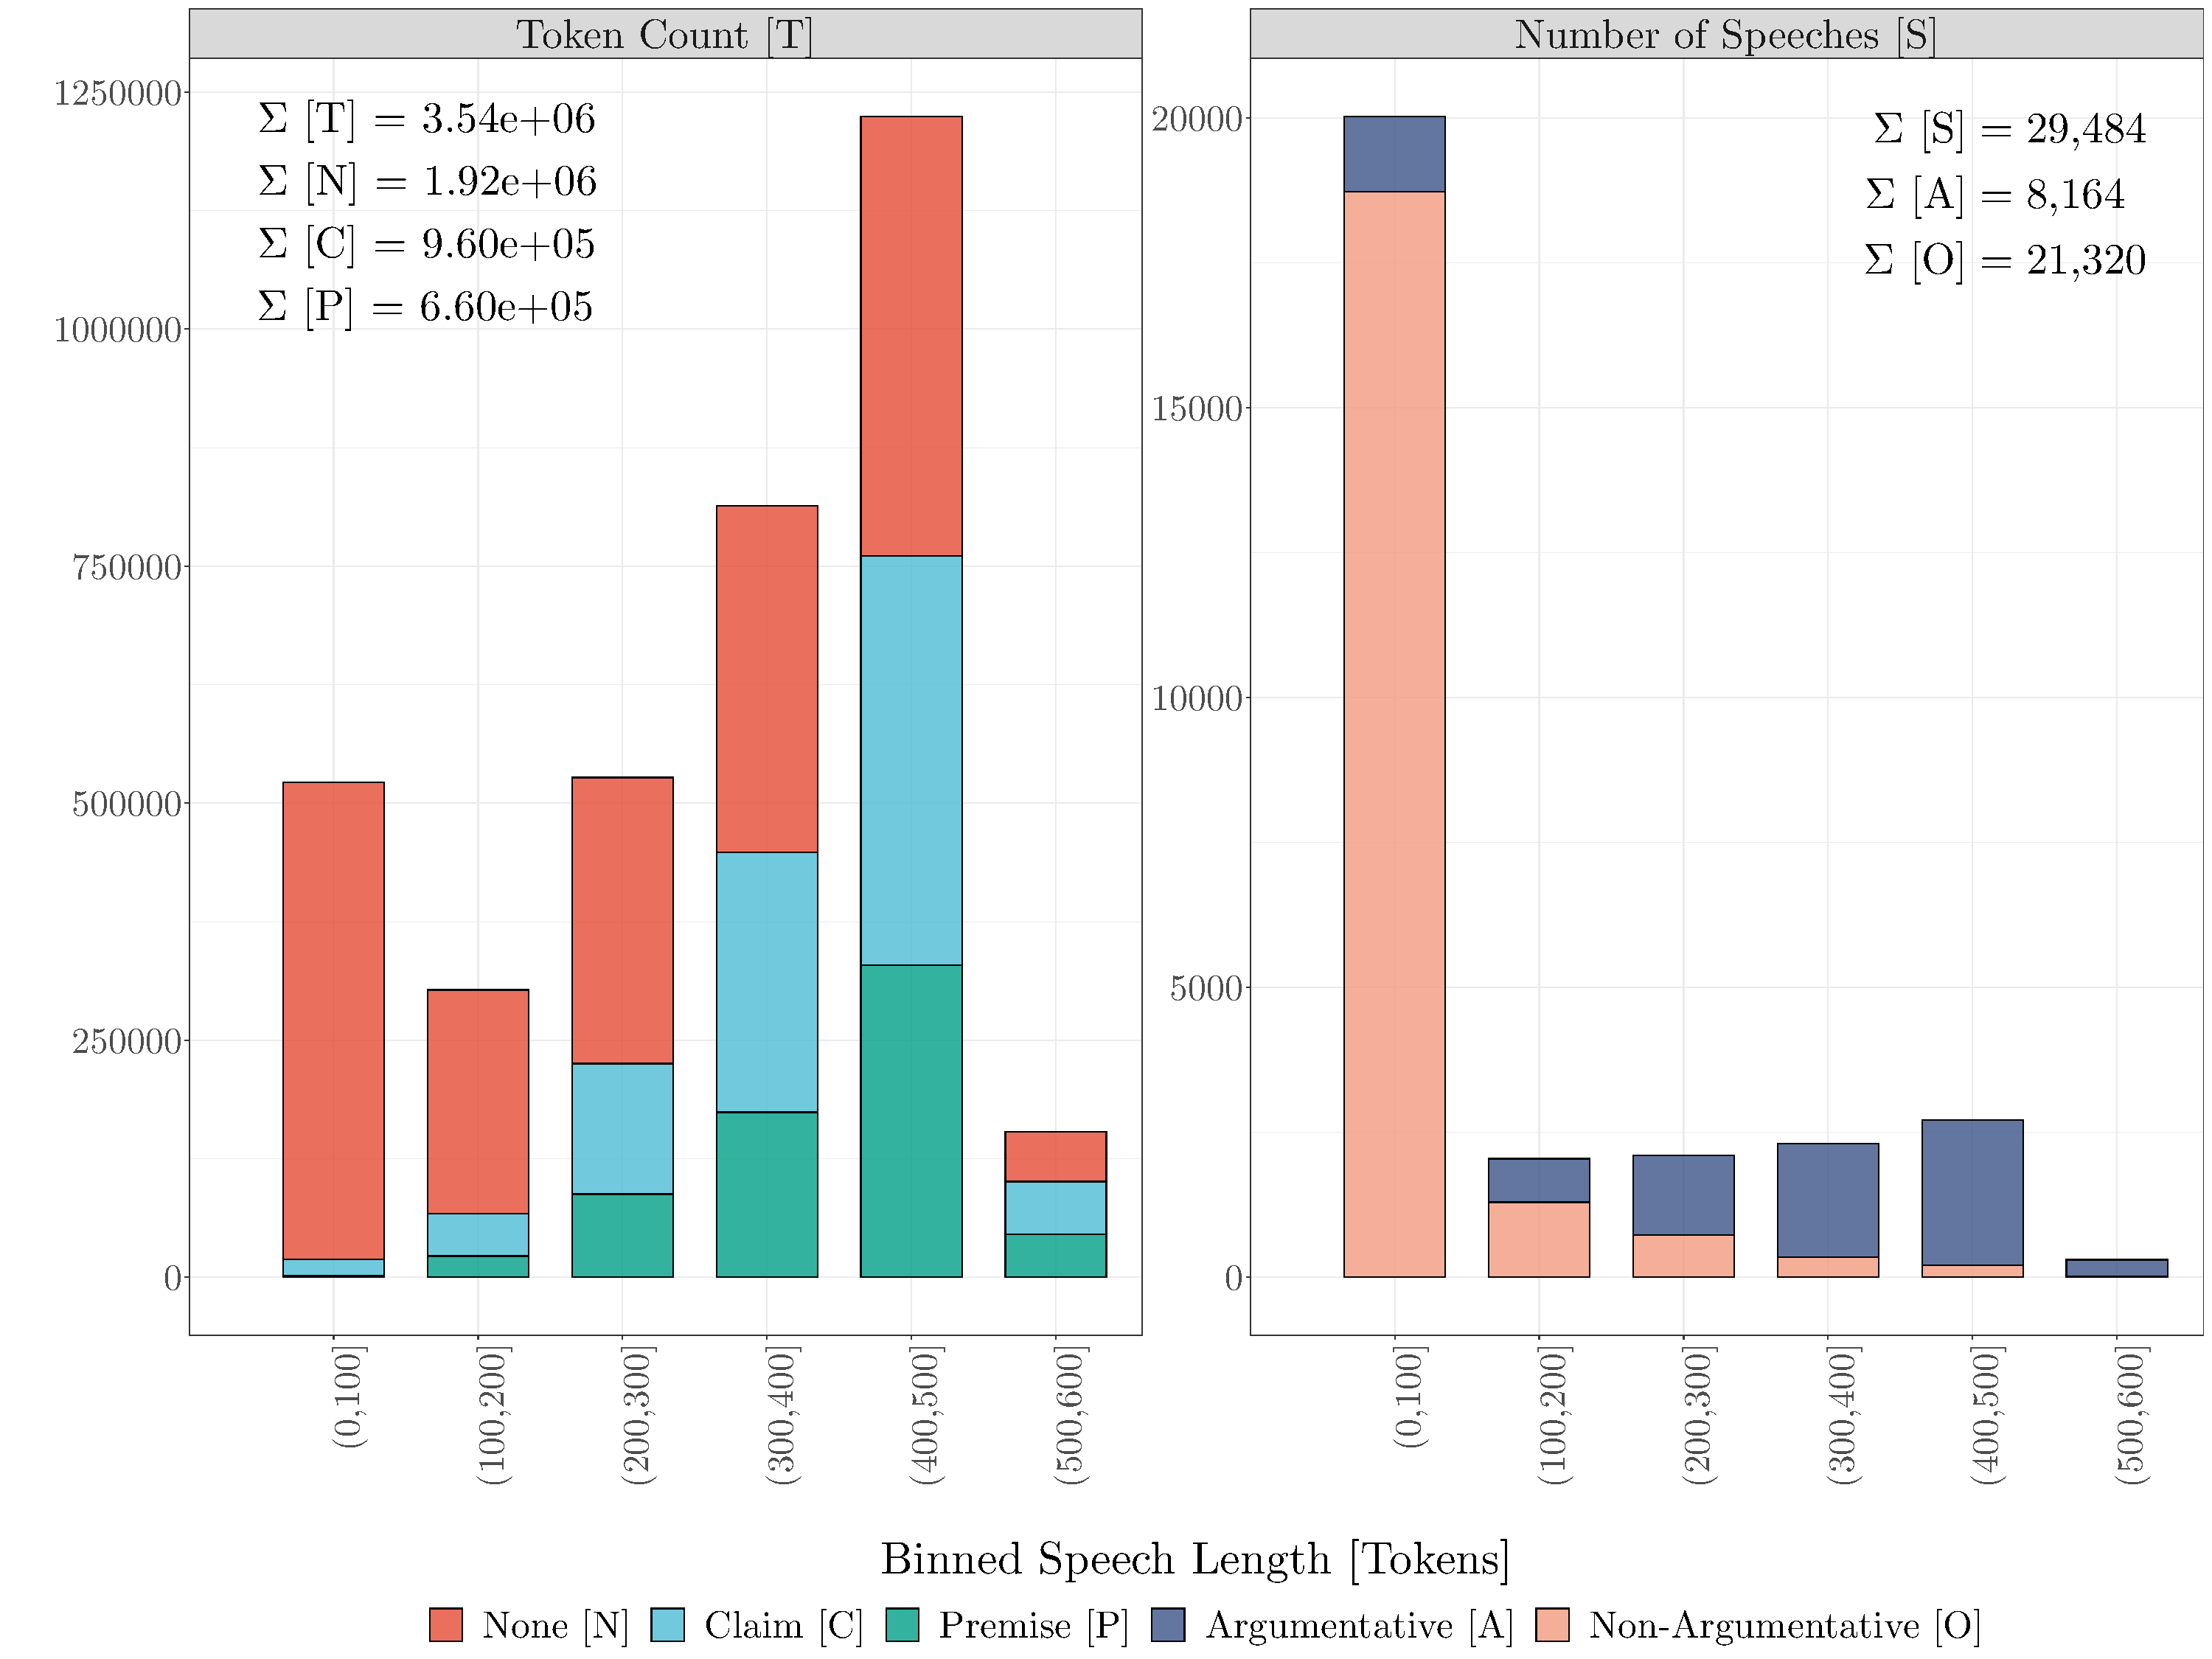
\includegraphics[trim={1.0cm 0cm 0cm
    0cm},clip,width=\textwidth]{img/token_dist_pred_UNSC_length.pdf}
    \caption{Token type predictions from TD$\_$Dense classifier on pruned UNSC corpus; non-argumentative (O) speeches have zero C and P tokens while argumentative (A) speeches contain at least one of either}
    \label{unsc_pred}
\end{figure}
\section{Discussion}
\label{discuss}

\subsection{Sentiment Analysis}
The results of the sentiment analysis seem to reveal a correlation of negative sentiment polarity and objectivity. The trend can be observed best in active countries for which we have a lot of data, e.g. the UNSC core nations and Germany. In order to confirm the validity of this correlation assumption, we would have to find viable means of evaluation. For this project, we manually evaluated a small number of speeches in order to get a grasp of the accuracy of our computed subjectivity and sentiment scores. The evaluation is not a simple task, as we are handling almost 65,000 speeches, and even evaluating 1\% of the data manually would be a labor-intensive tasks.

While performing the manual evaluation, we realized that the sentiment scoring yielded very positive results for rather neutral speeches. We also observed that the subjectivity scores were mostly located around the 0.5 mark, indicating the speech is somewhere in between objective and subjective. We assume that this is due to the fact that the United Nations Security Council speeches use unusual language. The English is very formal and lacks colloquial words and intensifiers. This kind of formal language, combined with the specific defense related topics discussed, might not be captured well by the two sentiment frameworks we used for the analysis. For the subjectivity scores, we came to the conclusion that due to the spokesperson speaking on behalf of an entire country, the typical indicators of subjective speech are not necessarily present, even if the spokesperson expresses their own opinion.

After close inspection of speeches from an extensive set of countries, we also noticed patterns that could have possibly lead to the high subjectivity polarity in some cases. It is part of the rules of etiquette to thank the previous speaker and in some cases elaborate on the positive work they did relating to a topic. At the end of speeches, the spokesperson or a moderator introduces the new person in a similar fashion. These sections of affirmation are repetitive and not related to the topics themselves, yet they are included in the scoring since they are part of the speeches. This skews the scores and raises the sentiment polarity to a higher level.
Furthermore, the speeches are oftentimes translated from the spokesperson's mother tongue to English, which can deprive the speeches of unique facets the speaker wanted to express since they can get lost in translation. 

One last aspect we noticed was that the speeches are stripped of environmental factors, e.g. interruptions that happened or hesitation on the part of the speaker. This would add valuable information to both levels of our analysis.

Despite the issues we noticed during the evaluation, we believe our sentiment analysis provides interesting insights into the UNSC speech data. While the results should be taken with a grain of salt, they still depict the differing sentiments among participants. Especially the insights into the Iraq War related sessions allow for an interesting digression into this controversial topic.

Said insights revealed for example that the opponents of this military intervention had a lower ratio of uttered negative vs. positive sentences than the proponents did. Even after a simple visual exploration of the plots, it is evident that the USA were the driving force in this issue, as they contributed the most to the sessions related to Iraq. Especially in the second session we analyzed, the session that opened with Colin Powell's speech, it can be seen that the two proponents of the invasion of Iraq, the USA and the UK, had a very negative vocabulary. While the UK did not contribute as much to the topic as the USA, more than 50\% of their contributions were negative. This degree of negativity cannot be observed in countries that held other opinions on the Iraq War. 

\subsection{Argumentation Mining}

\subsubsection{Model Performance Comparison}

Since the USED corpus is a relatively new political-domain argumentation corpus, we were unable to find directly comparable results from other studies. However, we can make some approximate comparisons from related studies. As mentioned in \ref{used}, \citet{haddadan-etal-2019-yes} performed argumentation classification of the USED corpus; albeit at a coarser sentence-level instead of the token-level. Their best model achieved 84.3$\%$ F$_1$ score for argumentative sentence identification and 67.3$\%$ F$_1$ score on claim/premise sentence classification. The better results could have stemmed from an intrinsically simpler sentence-level classification task.

\citet{eger2017neural} conducted a similar methodology as ours on the PEC; with their best model achieving a 75.6$\%$ F$_1$ score for the argumentation tagging task. This result is definitely a positive one, however we would question the robustness of such a model due to likely symbolic overfitting on the small training PEC containing only 402 essays.

\subsubsection{Prediction on UNSC}
\label{manual_semantic}

Due to time and resource limitations, we only manually review two predictions from our fine-tuned classifier on the UNSC corpus. We use the same coloring scheme for N, C and P tokens as per Figures \ref{used_distribution_combined} and \ref{unsc_pred}. In the positive example, we can observe clear and expansive segmentation with the claim and premise being in appropriate locations with a discourse connective ``but" between them. In the negative example, we can observe much more fragmentation of token spans; with the true premise after ``because" being (mostly) wrongly labelled as a claim. The fragmentation of token spans is not entirely surprising, since such fragmented argumentation spans also exist in the USED corpus. The true premise being wrongly predicted as a claim is however a limitation of the classifier in this example.

\begin{description}[style=nextline]

\item[\text{Positive Example: UNSC$\_$2004$\_$SPV.5007$\_$spch019}]
\colorbox{LightForestGreen}{\strut $\_$we} \colorbox{LightForestGreen}{\strut $\_$have} \colorbox{LightForestGreen}{\strut ,} \colorbox{LightForestGreen}{\strut$\_$indeed} \colorbox{LightForestGreen}{\strut ,} \colorbox{LightForestGreen}{\strut$\_$a} \colorbox{LightForestGreen}{\strut$\_$broad} \colorbox{LightForestGreen}{\strut$\_$range} \colorbox{LightForestGreen}{\strut$\_$of} \colorbox{LightForestGreen}{\strut$\_$tools} \colorbox{LightForestGreen}{\strut ,} \colorbox{LightForestGreen}{\strut$\_$developed} \colorbox{LightForestGreen}{\strut$\_$in} \colorbox{LightForestGreen}{\strut$\_$accordance} \colorbox{LightForestGreen}{\strut$\_$with} \colorbox{LightForestGreen}{\strut $\_$chapter} \colorbox{LightForestGreen}{\strut$\_$viii} \colorbox{LightForestGreen}{\strut$\_$of} \colorbox{LightForestGreen}{\strut$\_$the} \colorbox{LightForestGreen}{\strut$\_$charter} \colorbox{LightForestGreen}{\strut ,} \colorbox{LightForestGreen}{\strut$\_$to} \colorbox{LightForestGreen}{\strut$\_$facilitate} \colorbox{LightForestGreen}{\strut$\_$cooperation} \colorbox{LightForestGreen}{\strut .} \colorbox{red!60!white}{\strut$\_$but} \colorbox{LightCyan}{\strut$\_$we} \colorbox{LightCyan}{\strut$\_$need} \colorbox{LightCyan}{\strut$\_$fresh} \colorbox{LightCyan}{\strut$\_$ideas} \colorbox{LightCyan}{\strut$\_$in} \colorbox{LightCyan}{\strut$\_$order} \colorbox{LightCyan}{\strut$\_$to} \colorbox{LightCyan}{\strut$\_$improve} \colorbox{LightCyan}{\strut$\_$such} \colorbox{LightCyan}{\strut$\_$cooperation} \colorbox{LightCyan}{\strut$\_$and} \colorbox{LightCyan}{\strut$\_$to} \colorbox{LightCyan}{\strut$\_$make} \colorbox{LightCyan}{\strut$\_$sure} \colorbox{LightCyan}{\strut$\_$that} \colorbox{LightCyan}{\strut$\_$stability} \colorbox{LightCyan}{\strut$\_$can} \colorbox{LightCyan}{\strut$\_$be} \colorbox{LightCyan}{\strut$\_$achieved} \colorbox{LightCyan}{\strut$\_$as} \colorbox{LightCyan}{\strut$\_$a} \colorbox{LightCyan}{\strut$\_$result} \colorbox{LightCyan}{\strut$\_$of} \colorbox{LightCyan}{\strut$\_$cooperation} \colorbox{LightCyan}{\strut$\_$and} \colorbox{LightCyan}{\strut$\_$interaction} \colorbox{LightCyan}{\strut .}

\item [\text{Negative Example: UNSC$\_$2009$\_$SPV.6075$\_$spch042}]

 \colorbox{red!60!white}{\strut$\_$just} \colorbox{red!60!white}{\strut$\_$very} \colorbox{red!60!white}{\strut$\_$briefly} \colorbox{red!60!white}{\strut,} \colorbox{red!60!white}{\strut$\_$i} \colorbox{LightCyan}{\strut$\_$think} \colorbox{red!60!white}{\strut$\_$i} \colorbox{LightCyan}{\strut$\_$can} \colorbox{LightCyan}{\strut$\_$only} \colorbox{red!60!white}{\strut$\_$endorse} \colorbox{red!60!white}{\strut$\_$what} \colorbox{red!60!white}{\strut$\_$alain} \colorbox{red!60!white}{\strut$\_$le} \colorbox{red!60!white}{\strut$\_$roy} \colorbox{red!60!white}{\strut$\_$has} \colorbox{red!60!white}{\strut$\_$just} \colorbox{red!60!white}{\strut$\_$said} \colorbox{LightCyan}{\strut.} \colorbox{LightCyan}{\strut$\_$we} \colorbox{LightCyan}{\strut$\_$must} \colorbox{LightCyan}{\strut$\_$make} \colorbox{LightCyan}{\strut$\_$sure} \colorbox{LightCyan}{\strut$\_$that} \colorbox{LightCyan}{\strut$\_$we} \colorbox{LightCyan}{\strut$\_$commit} \colorbox{LightCyan}{\strut$\_$ourselves} \colorbox{LightCyan}{\strut$\_$fully} \colorbox{LightCyan}{\strut$\_$to} \colorbox{LightCyan}{\strut$\_$actively} \colorbox{LightCyan}{\strut$\_$participating} \colorbox{LightCyan}{\strut$\_$in} \colorbox{LightCyan}{\strut$\_$this} \colorbox{LightCyan}{\strut$\_$process} \colorbox{LightCyan}{\strut ,} \colorbox{red!60!white}{\strut$\_$because} \colorbox{LightForestGreen}{\strut$\_$we} \colorbox{LightForestGreen}{\strut$\_$all} \colorbox{LightCyan}{\strut$\_$see} \colorbox{LightCyan}{\strut$\_$that} \colorbox{LightCyan}{\strut$\_$the} \colorbox{LightCyan}{\strut$\_$outcome} \colorbox{LightCyan}{\strut$\_$of} \colorbox{LightCyan}{\strut$\_$such} \colorbox{LightCyan}{\strut$\_$a} \colorbox{LightCyan}{\strut$\_$good} \colorbox{LightCyan}{\strut$\_$dialogue} \colorbox{LightCyan}{\strut$\_$will} \colorbox{LightCyan}{\strut$\_$be} \colorbox{LightCyan}{\strut$\_$positive} \colorbox{LightCyan}{\strut$\_$for} \colorbox{LightCyan}{\strut$\_$our} \colorbox{LightCyan}{\strut$\_$missions} \colorbox{LightCyan}{\strut.}

\end{description}
\section{Conclusions}
\label{conclu}

In this project, we analyzed the UNSC corpus using two different approaches, sentiment analysis and argumentation mining. We aimed to provide automatic annotations for this novel political speech corpus, as it currently lacks hand-written annotations which would greatly facilitate the work of NLP researchers, as well as political scientists. We introduced the reader to the background concepts of our analyses and explained our methodologies. The detailed description of our results and their discussion shows that we succeeded in fulfilling our goals. We pointed to factors future researchers should bare in mind, for example state-of-the-art models and their limitations. Our final results and automatic annotations can be found in our GitHub repository\footnotemark[2].

While we do not provide definite and flawless annotations for the UNSC corpus, we succeeded in providing a well documented starting point for both sentiment and argumentation mining. We believe that the corpus can provide invaluable insights into the work and development of the United Nations Security Council and hope to have facilitated future research on this fascinating topic.

\section{Recommendations}
\label{reco}

 Given the resource and time limitations of our project, we were not able to perform extensive evaluations of our analyses. As this is fundamental for good scientific practice and the interpretation of results, we strongly recommend future researchers to employ an infrastructure for the evaluation of the produced annotations, e.g. by using crowdsourcing platforms. 
 
 As for the sentiment analysis, crowdsourcing manual annotations on word, n-gram or sentence level might also be an option worth considering. A partly annotated corpus would allow for machine learning analyses of the UNSC data and open up new perspectives. Furthermore, we think closer examination of specific subtopics might yield interesting results. Investigation of a subset of the corpus allows for a more fine-grained analysis and shows diverging opinions among countries better than a simple country-level analysis. Developing a strategy for identification and exclusion of non-relevant opening and closing words of speeches is also an open task that should be pursued.
 
 For argumentation mining, we could improve our training/validation and test data splits to create more homogeneous datasets. We could also attempt tagging tokens using the BIO scheme, as recommended by \citet{eger2017neural}, and check if that improves performance. In regards to fine-tuning, we recommend a transition from \texttt{TensorFlow} to \texttt{PyTorch} API's since there are more diverse collections of NLP-oriented deep-learning libraries which build upon the latter. Given limited hardware such as a single GPU, we would recommend memory-conserving training techniques such as gradient accumulation or checkpointing; which could allow for larger global batch-sizes and therefore less noisy gradients. We would also recommend multi-task training for the USED corpus with the second joint task being argumentation span linking using a graph neural network. Finally, we propose using different pre-trained language models which could handle multiple sentences better; such as XLNet, RoBERTa or Google's recently released Reformer (or efficient transformer) model.
\newpage
\addcontentsline{toc}{section}{References}
\bibliography{bibtex}
\bibliographystyle{apalike}
\nocite{*}
\end{document}

% final touches:
% TODO: truncate paper back to reasonable number of pages later on
% add paper to github with updates and linkages to bibtex and readmes3